\documentclass[12pt]{article}

\usepackage{cite}
\usepackage{listings}
\usepackage{multicol}
\usepackage{newtxtext}
\usepackage{setspace}
\usepackage{sectsty}
\usepackage{booktabs}
\usepackage{graphicx}
\usepackage{amsmath}
\usepackage{amssymb}
\usepackage{algorithm}
\usepackage{algpseudocode}
\usepackage{xcolor}
\usepackage{url}
\usepackage[T1]{fontenc}
% \usepackage[numbib]{tocbibind}
\usepackage[lmargin=1.25in,rmargin=1.25in,tmargin=1.0in,bmargin=1.0in]{geometry}

\definecolor{codegreen}{rgb}{0,0.6,0}
\definecolor{codegray}{rgb}{0.5,0.5,0.5}
\definecolor{codepurple}{rgb}{0.58,0,0.82}
\definecolor{backcolour}{rgb}{0.95,0.95,0.92}

\lstdefinestyle{thesiscodelisting}{
    keywordstyle=\color{magenta},
    numberstyle=\tiny\color{codegray},
    stringstyle=\color{green},
    basicstyle=\ttfamily\footnotesize,
    breakatwhitespace=false,
    breaklines=true,
    captionpos=b,
    keepspaces=true,
    showspaces=false,
    showstringspaces=false,
    showtabs=false,
}

\lstset{style=thesiscodelisting}

% \settowidth{\parindent}{}

\begin{document}
% Riddle thesis title page
\begin{center}
    \LARGE
    \textbf{
        \textit{
            Spoken Language Processing and Modeling for Aviation Communications\\
        }
    }

    \vspace*{0.2in}

    \normalsize
    by\\
    \textit{Aaron Van De Brook}\\

    \vspace*{0.25in}

\end{center}
This thesis was prepared under the direction of the candidate's thesis
committee chairman, \underline{Dr.~Jianhua Liu}, Department of \underline{Electrical Engineering \&
    Computer Science}, and has been approved by the members of the thesis committee.
It was submitted to the Department of Electrical Engineering \& Computer Science
and was accepted in partial fulfillment of the requirements for the degree of
Masters of Electrical \& Computer Engineering.

% Signature lines/committee members
\begin{center}
    \begin{minipage}{4.5in}
        \vspace*{0.35in}
        \hrule
        \vspace*{2pt}
        Jianhua Liu, Ph.D.\\
        Committee Chairman \& Graduate Program Coordinator \\
        \vspace*{0.5in}
        \hrule
        \vspace*{2pt}
        Prashant Shekhar, Ph.D.\\
        Committee Member\\
        \vspace*{0.5in}
        \hrule
        \vspace*{2pt}
        Andrew Schneider\\
        Committee Member\\
        \vspace*{0.5in}
        \hrule
        \vspace*{2pt}
        Massood Towhidnejad, Ph.D.\\
        Department Chair, Electrical Engineering \& Computer Science\\
        \vspace*{0.5in}
        \hrule
        \vspace*{2pt}
        James Gregory, Ph.D.\\
        Dean, College of Engineering\\
        \vspace*{0.5in}
        \hrule
        \vspace*{2pt}
        Christopher D.~Grant, Ph.D.\\
        Vice Provost of Academic Support\\
    \end{minipage}
\end{center}
\newpage
\tableofcontents
\newpage
\doublespacing{}

\section{Abstract}\label{sec:abstract}
With recent advances in machine learning and deep learning technologies and the creation of larger aviation-specific corpora, applying
natural language processing technologies, especially those based on transformer neural networks, to aviation communications is becoming
increasingly feasible. Previous work has focused on machine learning applications to natural language processing, such as N-grams and
word lattices. This thesis experiments with a process for pretraining transformer-based language models on aviation English corpora and
compare the effectiveness and performance of language models transfer learned from pretrained checkpoints and those trained from their
base weight initializations (trained from scratch). The results suggest that transformer language models trained from scratch outperform
models fine-tuned from pretrained checkpoints. The work concludes by recommending future work to improve pretraining performance and
suggestions for downstream, in-domain tasks such as semantic extraction, named entity recognition (callsign identification), speaker
role identification, and speech recognition.

\section{Introduction}\label{sec:introduction}
There have been noticeable and significant advancements in the general domain of artificial intelligence (AI) recently. Natural
language processing and language modeling technologies, in particular, have made tremendous advances over the past two decades
\cite{hannun_deep_2014,lee_unsupervised_2009,li_jasper_2019,kriman_quartznet_2020}, achieving performance levels good enough to be brought to
consumer-facing products such as personal assistants, search engines, phones, televisions, etc. Due to the success in the general domain, applications
have begun to spin off into problem-specific domains, such as (and most notably for this work) aviation. For example, several speech recognition
systems with rule- and machine learning-based natural language processing, inference, and semantic extraction algorithms have been implemented at
EUROCONTROL simulation centers in Europe to train air traffic controllers and study the potential effects of AI-augmented air traffic management (ATM)
systems on controller workloads \cite{helmke_quantifying_2017,helmke_assistant-based_2015}. Preliminary studies have found that AI-augmented ATM
systems reduce controller workloads and fuel consumption of aircraft by optimizing aircraft routes in the airspace and reducing departure/arrival
times, thereby reducing fuel consumption \cite{helmke_quantifying_2017}.

At the time of this writing, the current focus of general machine learning and deep learning algorithms in the language modeling domains has been on a
variety of deep learning methods/architectures, namely, recurrent, convolutional, and transformer neural networks, due to the availability of large
natural language corpora such as WikiText \cite{merity_pointer_2016} and IMDB \cite{maas_learning_2011}. In contrast to the general domain, the
aviation domain still prefers and sees much success with traditional machine learning models for language modeling applications. Typically, the most
prevalent of the traditional models are N-grams, word lattices, and rule-based approaches, depending on the application and operating environment of
the models. The most likely reason for this divergence between the domains is the difference and relative lack of labeled data in the aviation domain.
By comparison, the largest corpora in the general domain are either WikiText or the BookCorpus, which contain trillions of tokens, whereas, for
aviation, the largest corpus is Air Traffic Control Complete with approximately 26 hours of labeled data amounting to just over 300,000
tokens\footnote{Air Traffic Control Complete has approximately 70 hours of audio data, however, about 26 hours of the 70 are labeled.}. This disparity
in data availability is exacerbated by the fact that aviation English uses a specialized vocabulary in addition to specialized pronunciation for some
words to enhance understandability in a radiotelephonic (R/T) medium \cite{paltridge_handbook_2013}. This makes the data labeling process
significantly more difficult because it not only requires two types of data (audio and text) to create labels, but also requires labelers to have
domain knowledge and experience to create effective transcriptions. This, in addition to the following facets, further contributes to the difficulty
of transcription: (1) the medium of communication, (2) the environment in which the communication occurs\footnote{For example, a noisy and possibly
    low fidelity medium, depending on the equipment used to transmit and receive communications}, (3) a noisy and active communication environment
i.e.~an active flight deck under the influence of wind, engine noise, etc., (4) an active Air Traffic Control (ATC) tower and channels contributing to
increased background noise on the ATC side, and (5) a rapid rate of speech. Pilots are also operating sophisticated equipment during while
communicating, requiring significant attention and mental resources further contributing to the complexity of the communications
\cite{paltridge_handbook_2013}.

% connect complexity of aviation english to utility/necessity of NLP models (ASR and LM) in the aviation domain
The potential for speech recognition and language modeling algorithms to reach better than human performance (for example, the Stanford Question
Answering Dataset (SQuAD) benchmark has recorded results consistently better than humans since
2019\footnote{\url{https://rajpurkar.github.io/SQuAD-explorer/}}) \cite{zhang_ai_2022} suggests that these NLP algorithms could have high utility in the
aviation domain. If they can achieve better-than-human performance in the aviation domain and be used with pilot and air traffic controller systems,
they could easily boost efficiency, reduce workloads, and reduce and mitigate errors during normal operations.

The methods and results laid out in this thesis were done with the intention of creating a streamlined process for training and testing deep
learning-based NLP methods, specifically language modeling. The results from the language models suggest that the volume of text used to train the
language models is not yet sufficient to produce results akin to those in the conversational and/or literary English domains. Additionally, the
results in Section \ref{sec:results_comparison} show that language models trained ``from scratch'' on in-domain data perform better than models
trained on out-of-domain data and transfer learned on in-domain data.

\subsection{Problem Statement}\label{sec:problem_statement}
Other work has shown that the word error rates of automatic speech recognition models can and have been significantly reduced by using language models
to determine the most likely token at a time step in a sequence \cite{li_jasper_2019,kriman_quartznet_2020}. Language models have also been shown to
be effective for natural language processing tasks such as named entity recognition \cite{devlin_bert_2019,liu_roberta_2019}. Speech recognition and
callsign detection (CSD) have become popular tasks for machine learning applications in aviation
\cite{pellegrini_airbus_2019,delpech_real-life_2018,helmke_quantifying_2017}; callsign detection is a task analogous to named entity recognition since
the elements of a callsign in a transcription can be treated as named entities in a sentence. For example, in the following transcription

\begin{quote}
    skyshuttle one one four zero now descend flight level three three zero
\end{quote}

\noindent
the sequence ``skyshuttle one one four zero'' should be detected as the callsign. This is similar to detecting ``EU'', ``German'', and ``British'' as
named entities in the sequence below.

\begin{quote}
    EU rejects German call to boycott British lamb
\end{quote}

The key component missing for both of these applications is an effectively pretrained language model that can be used for these downstream tasks, so
the goal of this thesis is to run several experiments using transformer-based language models to determine the most effective strategy for pretraining
the model for downstream tasks. Recommended best practice is to use a pre-existing language model checkpoint and fine-tune on additional data
\cite{devlin_bert_2019,liu_roberta_2019,lewis_bart_2019}, although recent work suggests that if domains are sufficiently different, the performance
of the fine-tuned model will be limited \cite{yadlowsky_pretraining_2023}. The main point of comparison in this thesis will be the performance of
pretrained models fine-tuned on in-domain (aviation) data and models trained from scratch on in-domain data. The experiments and results presented in
this thesis are preliminary applications of end-to-end deep learning solutions to Automatic Speech Recognition (ASR) and Natural Language Processing
(NLP) problems in aviation. The intention is for this work to provide knowledge and possibly checkpoints for the ASR and language models which can be
used for downstream tasks such as callsign detection and beam search prediction decoding for ASR models.

\subsection{Notation \& Terminology}
This section is included for the sake of clarity throughout this thesis. In pursuit of that, a few terms and notations are defined below.

Set notation (or set-builder notation)\footnote{That is, the notation used to denote sets and associated operations therein as it relates to the field
    of set theory, in mathematics.} as defined in \cite{jech_chapter_1978} is used in parts of this thesis, particularly in equations and algorithms,
to convey mathematical concepts. The shorthand below is defined
\begin{equation*}
    A; x := A \cup \{x\}
\end{equation*}

\noindent
as the union of the set $A$ and a set containing the element $x$. The equation below can be read as adding the element $x$ to the set $A$:

\begin{equation*}
    A \leftarrow A; x
\end{equation*}

The following words (in bold) are used throughout the thesis as they relate to language modeling and are defined concretely as follows:

The definition of words and sentences stem from their definitions in the English language, succinctly, as defined in \cite{noauthor_american_2011}:

\begin{itemize}
    \item A \textbf{word} is the representation in writing of a sound or combination of sounds that symbolizes and communicates a meaning.
    \item A \textbf{sentence} is a grammatical unit that is syntactically independent that is expressed or understood and contains at least one finite
          verb.
\end{itemize}

\noindent
In terms of the structure of individual samples in a corpus, we will consider each sample in the corpus to be one sentence that is made up of words
that are separated by whitespace (one or more spaces) and/or punctuation. Structurally, we consider a word to be made up of one or more characters
as defined by the unicode standard \cite{allen_unicode_2012} and a sentence to be made up of one or more words.

\begin{itemize}
    \item A \textbf{token} shall be defined as the smallest, fundamental component of a sequence; these can be single characters, groups of
          characters, punctuation, etc. \cite{devlin_bert_2019,wu_googles_2016,sennrich_neural_2016}
    \item A \textbf{sequence} shall be defined as a set of tokens (distinct from a sentence).
\end{itemize}

\noindent
As mentioned above, we consider each \textbf{sample} in a corpus to be a sentence, then as the corpus is collated, processed, and tokenized, each
sample will be processed into sequences of tokens. These sequences are what will be analyzed and modeled by the language models.

The rules by which words in sentences are broken up into tokens are defined by tokenization algorithms, otherwise known as tokenizers (elaborated
further in Section \ref{sec:tokenizers}). While tokens can be individual characters or words as they appear in the original sample, this is not always
the case. The intention of most tokenization algorithms is the flexibility to break up unknown words into smaller tokens known to the tokenizer
\cite{wu_googles_2016,sennrich_neural_2016}.

\section{Background \& Literature Review}\label{sec:lit_review}

\subsection{Transformer Neural Networks}
% from thesis proposal; revise and add to this as more references are used
% transformer history (background)
The transformer neural network architecture (shown in Figure \ref{fig:transformer_arch}) was proposed in 2017 for Neural Machine Translation tasks and
immediately achieved state-of-the-art performance on language translation tasks \cite{vaswani_attention_2017}. Transformer architectures are extremely
effective at learning representations and understandings of languages to predict token probabilities instead of transforming one language into another
\cite{devlin_bert_2019,liu_roberta_2019}. Transformers have also been found to be very effective at other NLP tasks such as prompt completion
and sentiment analysis among others (i.e.~auto-regressive and sequence classification tasks, respectively)
\cite{lewis_bart_2019,radford_improving_2018}. Devlin et al.~\cite{devlin_bert_2019} proposed pretraining methods such as masked language modeling
and next sentence prediction to improve natural language understanding for downstream tasks, which was further expanded upon by Liu et
al.~\cite{liu_roberta_2019} by training longer, with larger batch sizes, and removing the next sentence prediction task.

\begin{figure}[!t]
    \centering
    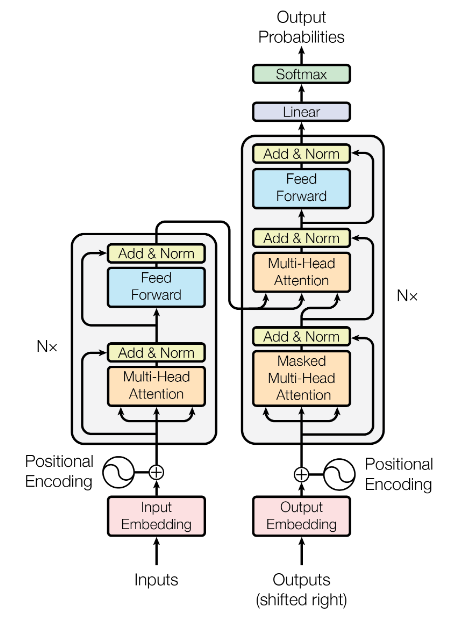
\includegraphics[width=0.5\linewidth]{figures/transformer_arch.png}
    \caption{The transformer neural network architecture. Copied from page 3 of Vaswani et al.~\cite[Fig. 1]{vaswani_attention_2017}}
    \label{fig:transformer_arch}
\end{figure}

\subsection{Tokenizer Algorithms}
% tokenizer algorithms
In language modeling and natural language processing tasks, the out-of-vocabulary (OOV) problem is prevalent and has been addressed by the
introduction of tokenizer algorithms. WordPiece and Byte Pair Encoding (BPE) have been used to solve OOV problems while simultaneously minimizing
vocabulary sizes and maximizing the likelihood of tokens in sequences \cite{wu_googles_2016,schuster_japanese_2012,sennrich_neural_2016}.

\subsection{Language Modeling \& Natural Language Processing in Aviation}
% LMs and NLP in aero. domain
Various natural language processing methods have been applied to the aviation domain to help deal with miscommunications and try to mitigate safety
incidents\cite{ragnarsdottir_language_2003,tanguy_natural_2016,madeira_machine_2021}. Some machine learning approaches have been implemented to
analyze the text in aviation incident and safety reports to predict contributing factors and topic models
\cite{tanguy_natural_2016,madeira_machine_2021}. An ASR system with NLP post-processing has also been proposed to analyze Air-Traffic communications
and condense significant features (e.g.~weather, runway, and heading info) into an XML language structure\cite{ragnarsdottir_language_2003}.
Transformer language models such as BERT and RoBERTa have been applied to notice to airmen (NOTAM) messages to perform named entity recognition (NER)
tasks, translation tasks (between notations; e.g.~NOTAM notation to Airlang to make parsing tasks easier) and reduce the workload for pilots during
long-haul flights\cite{arnold_knowledge_2022}. Transformer models have also been used for speaker role identification tasks in the aviation domain
(e.g.~identifying pilot versus controller in communications); specifically, a pretrained BERT model was used and fine-tuned on problem-specific data
and compared to other models that performed well at speaker and role identification tasks in general\cite{guo_comparative_2022}.

\subsection{Automatic Speech Recognition in Aviation}
% ASR context (suggest some need for semi-supervised approaches and therefore LMs)
Automatic speech recognition (ASR) is seeing increased use in aviation for tasks such as transcription, callsign detection, speaker identification, etc. A
majority of these approaches use machine learning approaches (as opposed to deep learning) where acoustic, pronunciation, and language modeling is
used to transcribe speech
\cite{guo_comparative_2022,smidl_air_2019,zuluaga-gomez_automatic_2020,badrinath_automatic_2022,hofbauer_atcosim_2008,helmke_quantifying_2017}.
Language models have been used in the general domain (both neural and machine learning-based approaches) to boost the performance of speech
recognition models \cite{han_contextnet_2020,kriman_quartznet_2020,majumdar_citrinet_2021}. Machine learning-based language models, usually N-grams
and word lattices, have also been used in aviation alongside semi-supervised approaches to automatic speech recognition to leverage unlabeled data.
However, none of the developed methodologies use neural language models for their applications
\cite{zuluaga-gomez_contextual_2021,srinivasamurthy_semi-supervised_2017,badrinath_automatic_2022}.

ASR and speech synthesis technologies have seen use for improving communications and reducing pilot workload as early as 1981
\cite{money_aural_1981,north_application_1984,north_systems_1984,mayer_electronic_1981}. Early approaches focused on developing and improving speech
synthesis technologies to shift pilot focus in military and general aviation cockpits to urgent systems or alarms
\cite{mayer_electronic_1981,money_aural_1981,mosko_clear_1981}. ASR system concepts and technologies were also initially developed to reduce pilot
workloads and automate simple tasks; these systems were somewhat rigid with fixed vocabularies and keywords, but were able to successfully reduce
workload and received positive feedback from pilots \cite{north_application_1984,cotton_development_1983}. Similar ASR technologies were later applied
to Air Traffic Control (ATC) contexts to reduce controller workloads and increase the efficiency of Air Traffic Management (ATM) solutions
\cite{schafer_context-sensitive_2000,lechner_voice_2002,ragnarsdottir_language_2003,cordero_automated_2012}. As ASR technologies have become more
sophisticated and more aviation-specific speech corpora have become available
\cite{godfrey_air_1994,smidl_air_2019,hofbauer_atcosim_2008,szoke_detecting_2021,segura_hiwire_2007,graglia_vocalise_2005,delpech_real-life_2018,zuluaga-gomez_atco2_2023}
there have been more applications of ASR to aviation
\cite{moere_implementing_2009,gurluk_assistant_2015,helmke_assistant-based_2015,helmke_machine_2020,helmke_readback_2021,kleinert_automated_2021,badrinath_automatic_2022,shi_end--end_2022,xiao_speech_2022,zuluaga-gomez_atco2_2023}.


\subsection{Differences in Language}
% differences in language (aviation vs casual english), narrow model selection
The use of the English language in aviation has been shown to be sufficiently different enough to be classified under its own category (aviation
English) \cite{paltridge_handbook_2013}. The issue with using pretrained checkpoints of transformer-based language models is characterizing the
similarity (or, conversely, the difference) between casual and technical English i.e., in this case, the differences between written English, as in
books and articles, and the spoken, transcribed English used in aviation. If the two domains are sufficiently different, then training the pretrained
models on aviation English data would amount to transfer learning between specific domains. Transfer learning between text domains has been shown to
be possible even with data volumes significantly lower than the original data used to train the models \cite{raffel_exploring_2020}. Yadlowsky et
al.~\cite{yadlowsky_pretraining_2023} recently showed that if problem domains are sufficiently different, model pretraining on out-of-domain data will
negatively affect model performance.

\section{Datasets \& Preparation}\label{sec:data_source}
Four corpora are combined and used for the experiments in this thesis. The datasets are primarily speech corpora intended for automatic speech
recognition research in aviation communications, linguistics research in aviation English, or both. All data in all four corpora include both
recordings and transcriptions, which are audio and text, respectively. The transcriptions are used to pretrain and train the language models and
tokenizers (described in sections \ref{sec:language_models} and \ref{sec:tokenizers}).

The four corpora selected and used for this work are briefly described below. Further analysis is performed in Section \ref{sec:data_analysis}.

\subsection{Air Traffic Control Complete}\label{sec:atcc}
The Air Traffic Control Complete (ATCC) corpus is a speech corpus consisting of audio recordings with corresponding transcriptions. ATCC is a
collection of three smaller corpora recorded at Dallas-Fort Worth, Logan International, and Washington National airports and transcribed by current or
former air traffic controllers familiar with the respective areas. Audio data was recorded by placing Very High Frequency (VHF) antennae configured to
monitor several frequencies at each airport, such as arrival, departure, approach, ground, etc. The types of frequencies observed vary by airport, but
the presence of departure, approach, and ground frequencies is relatively consistent across subcorpora \cite{godfrey_air_1994}. See Table
\ref{tab:atcc_stats} for corpus-specific statistics.

\begin{table}[!t]
    \centering
    \begin{tabular}{l r}
        \toprule
        \multicolumn{2}{c}{ATCC Corpus Properties} \\
        \midrule
        Samples              & 9,556               \\
        Audio (hours)        & 72.48               \\
        Mean Sequence Length & 11.90               \\
        Std.~Sequence Length & 7.22                \\

        Total Tokens         & 355,485             \\
        Unique Tokens        & 2,209               \\
        \bottomrule
    \end{tabular}
    \caption{Data statistics for the Air Traffic Control Complete (ATCC) corpus.}
    \label{tab:atcc_stats}
\end{table}

\subsection{ATCO2}\label{sec:atco2}
The ATCO2 dataset is a speech corpus comprising audio communications at Prague and Brno airports in Czechia and corresponding transcriptions. The
speech recordings and transcripts are crowd-sourced from volunteers. The dataset was created and labeled, in part, as an English language detection
corpus. However, the labeling also includes transcripts of speech segments, which makes it practical for ASR and language model development in
addition to language detection (although in this work, it is only used for ASR and LM development)~\cite{szoke_detecting_2021}.
See Table \ref{tab:atco2_stats} for corpus-specific statistics.

\begin{table}[!t]
    \centering
    \begin{tabular}{l r}
        \toprule
        \multicolumn{2}{c}{ATCO2 Corpus Properties} \\
        \midrule
        Samples              & 874                  \\
        Audio (hours)        & 1.10                 \\
        Mean Sequence Length & 12.28                \\
        Std.~Sequence Length & 5.78                 \\
        Total Tokens         & 10,733               \\
        Unique Tokens        & 786                  \\
        \bottomrule
    \end{tabular}
    \caption{Data statistics for the ATCO2 corpus.}
    \label{tab:atco2_stats}
\end{table}

\subsection{Air Traffic Control Simulation}\label{sec:atcosim}
The Air Traffic Control Simulation (ATCOSIM) corpus is a speech corpus consisting of audio recordings and corresponding transcriptions. The data was
recorded at the EUROCONTROL Experimental Centre for air traffic control simulation in Bretigny-sur-Orge, France. In this corpus, only the controllers'
voices are included, and therefore, the transcripts only include the controller's side of each interaction. The audio data was transcribed by one
person, trained according to the guidelines and formatting requirements of the corpus. After all data was transcribed, it was reviewed and corrected,
and any remaining problems were reviewed by an operational air traffic controller and resolved \cite{hofbauer_atcosim_2008}. See Table
\ref{tab:atcosim_stats} for corpus-specific statistics.

\begin{table}[!t]
    \centering
    \begin{tabular}{l r}
        \toprule
        \multicolumn{2}{c}{ATCOSIM Corpus Properties} \\
        \midrule
        Samples              & 9,556                  \\
        Audio (hours)        & 10.69                  \\
        Mean Sequence Length & 11.29                  \\
        Std.~Sequence Length & 4.17                   \\
        Total Tokens         & 107,881                \\
        Unique Tokens        & 827                    \\
        \bottomrule
    \end{tabular}
    \caption{Data statistics for the ATCOSIM corpus.}
    \label{tab:atcosim_stats}
\end{table}

\subsection{ZCU CZ ATC Corpus}\label{sec:zcu_atc}
The ZCU CZ ATC corpus consists of audio recordings and corresponding transcripts in the Czech airspace. Both the controller and pilot sides of the
communications are included in this data. Experienced transcribers/annotators created annotations, and labeled samples were randomly selected for
review during the annotation process. After the dataset was completely labeled, all samples were checked, corrected, and unified\cite{smidl_air_2019}.
See Table \ref{tab:zcu_cz_atc_stats} for corpus-specific statistics.

\begin{table}[!t]
    \centering
    \begin{tabular}{l r}
        \toprule
        \multicolumn{2}{c}{ZCU CZ ATC Corpus Properties} \\
        \midrule
        Samples              & 14,435                    \\
        Audio (hours)        & 20.58                     \\
        Mean Sequence Length & 10.05                     \\
        Std.~Sequence Length & 5.50                      \\
        Total Tokens         & 145,107                   \\
        Unique Tokens        & 3,100                     \\
        \bottomrule
    \end{tabular}
    \caption{Data statistics for ZCU CZ ATC corpus.}
    \label{tab:zcu_cz_atc_stats}
\end{table}

\subsection{Data Preparation}\label{sec:data_preparation}
All corpora listed above (see Section \ref{sec:data_source}) are created at different times, for various purposes, and by multiple authors. As a
result, the data in these corpora all have different formats. ATCC, for example, uses Lisp-style lists as below:

\begin{lstlisting}
((FROM NERA3788) (NUM L02F1-0001)
(TO F1-1)
(TEXT THOUSAND ONE NINETY WE (QUOTE LL) GIVE YOU THAT ON THE SPEED AND WE (QUOTE RE) CLEARED FOR THE APPROACH AH NERA THIRTY SEVEN EIGHTY EIGHT WE (QUOTE LL) HOLD SHORT OF TWO SEVEN)
(TIMES 1.49 6.57))
\end{lstlisting}

ATCO2 and ZCU CZ ATC use XML to isolate transcribed segments of speech in the audio recordings, although the format used between the two differs.
ATCO2 uses a form like below:

\begin{lstlisting}
<data>
<segment>
<start>3.79</start>
<end>6.85</end>
<speaker>B</speaker>
<speaker_label>OK-PMB</speaker_label>
<text>level one hundred Oscar Kilo Papa Mike Bravo</text>
<tags>
<correct>0</correct>
<correct_transcript>1</correct_transcript>
<correct_tagging>0</correct_tagging>
<non_english>0</non_english>
</tags>
</segment>
</data>
\end{lstlisting}

ZCU CZ ATC uses a different nesting and labeling style, like below\footnote{Some information is excluded for readability.}:

\begin{lstlisting}
<Trans audio_filename="e2_ACCU-0agmXf.wav">
<Episode>
<Section type="report" startTime="0" endTime="61.47">
<Turn startTime="0" endTime="61.47">
<Sync time="0.000"/>
[ground]Skyshuttle 1 1 4 0 now descend FL 3 3 0[speaker]
<Sync time="4.790"/>
[air]descending FL 3
<Sync time="6.650"/>
[air]K O Z
<Sync time="9.640"/>
[ground_|]Austrian 3 2 3 G climb FL 3 4 0 [|_ground][air_|]level 3 4 0 Austrian 3 2 3 G[|_air]
</Turn>
</Section>
</Episode>
</Trans>
\end{lstlisting}

Lastly, ATCOSIM uses a text-only format with transcriptions occurring on their own lines in text files:

\begin{lstlisting}
[FRAGMENT] contact geneva one two eight decimal one five good bye
\end{lstlisting}

\noindent
Each text file corresponds to the audio file from which the speech was transcribed.

Due to the differing formats above, and the intention to aggregate and use all these transcripts together, all transcripts need to be processed into
a common format to be used together.

All data was processed in Python using primarily built-in functions/modules\footnote{The \lstinline|re| and \lstinline|xml| modules were also used,
    although these are built into most Python distributions by default.}. The text data is extracted from the corpus transcripts by reading each
transcript into the main memory of the system according to the format prescribed by the corpus. The text corresponding to the transcript is isolated,
copied, and stored to a separate region of memory (a Python list of strings) that corresponds to the original corpus. The resulting isolated
transcripts are written to files that correspond to the original corpus as well as combined, shuffled, and written to a file in the standard corpus
format (an ASCII text file with one line in the file corresponding to one sample from the corpus). The resulting output is four corpus files that
correspond to the original corpora in addition to a fifth corpus file with the samples from all four corpora combined and shuffled for later
use\footnote{See the \lstinline|parse_transcripts| functions in the files at \url{https://github.com/AVanDeBrook/msece-thesis/tree/main/source/data}
    for implementation details.}.

\subsection{Handling Spelling Errors \& Inconsistencies}\label{sec:spelling_errors}
By the nature of the data labeling process, there is a high likelihood of spelling errors introduced by the annotators during corpora creation. This
gets exacerbated by aggregating several corpora with varying controls for correcting spelling errors and inconsistencies. Nearly all of the mistakes
are recoverable/correctable, given proper context. For example, ``possibility of \textbf{tornado's}'' should have been ``possibility of
\textbf{tornadoes}'', changing the possessive form of ``tornado'' to the plural form. There are also instances of spelling conventions that are
consistent within corpora but become inconsistent when combined.

% 22 spelling errors
Manually reviewing every sample in the corpus is unrealistic, considering that there are over 50,000 data samples and would be subject to the same
human error that introduced those errors in the first place. Instead, the frequency of token occurrence in the corpora, combined with manual review
thereafter, was used to detect and correct the most common errors. Tokens with the lowest frequency across corpora (and lowest number of occurrences)
were manually reviewed and corrected where necessary. Tokens that needed to be corrected typically occurred five times or less per corpus although
all tokens with occurrences ranging from 1-50 were reviewed. The relative frequency of those tokens varies by corpus (due to the differing amont of
tokens in total for each corpus) The frequency of occurrence of a token is calculated using equation (\ref{eq:token_frequency_occurrence}), below

\begin{equation}\label{eq:token_frequency_occurrence}
    f_w = \frac{\phi_w(w)}{D_{tokens}}
\end{equation}

\noindent
where $f_w$ is the frequency at which a token occurs in a corpus, $\phi_w(w)$ is the number of times a token, $w$, occurs, and $D_{tokens}$ is the
total number of tokens in the corpus.

An $A \rightarrow B$ mapping system was used to correct the errors, where \(A\) is the erroneous token and \(B\) is the
corrected or replaced token. As the text is parsed from the corpora, each sample is analyzed. If an erroneous token, $A$, is found, it is replaced
with the corrected version, $B$. 22 unique errors were detected and subsequently corrected or removed using this method. However, multiple instances
of those errors typically occurred.

% hesitations, cut off words, different kinds of filled pauses
The mapping system described above is also used to make corpora conventions to be consistent across corpora. Three areas are addressed here:
hesitations, cut-off, or partial words, and filled pauses within speech. These areas are defined differently between the four corpora, which makes
unifying the transcripts difficult. Hesitations, for example, are defined by one corpus as incomplete or non-English speech sounds and left completely
undefined by another (despite annotators making notes about hesitations). The way in which hesitations, pauses, and partial words are transcribed
differs between corpora as well. Two corpora prescribe special tokens to these phenomena, such as ``[hes]'', ``[hesitation]'', ``<pause>'', or
similar. In contrast, the others transcribe the data as it sounds (i.e., ``uh'', ``eh'', or ``er'' for filled pauses and ``cir-'' or ``cir+'' for
instances that were cut-off mid pronunciation). To facilitate the unification of the transcripts for all four corpora, the conventions for
transcribing these phenomena are redefined in Table \ref{tab:phenomena_definitions}.

\begin{table}[!t]
    \centering
    \begin{tabular}{l p{0.65\linewidth}}
        \toprule
        Phenomenon               & Definition                                                                                                                \\
        \midrule
        Hesitations              & Instances of spoken words for which the specific realization is not defined (usually some special token is used instead). \\
        \midrule
        Partial \& cut-off words & Partially pronounced words are indicated by a hyphen character where the pronunciation of the word is missing.            \\
        \midrule
        Filled pauses            & Hesitations with a verbal component that has been described or otherwise defined by the corpus/annotator.                 \\
        \bottomrule
    \end{tabular}
    \caption{Speech/transcription phenomena with corresponding convention for transcribing or translating, depending on the corpus being processed.}
    \label{tab:phenomena_definitions}
\end{table}


\begin{table}[!t]
    \centering
    \begin{tabular}{l l}
        \toprule
        Phenomenon                   & Convention for representation \\
        \midrule
        Hesitations                  & [HES]                         \\
        \midrule
        Partial \& cut-off words     & -                             \\
        \midrule
        Filled pauses (open-mouth)   & uh, um, ah                    \\
        \midrule
        Filled pauses (closed-mouth) & hm, mhm                       \\
        \bottomrule
    \end{tabular}
    \caption{Conventions for transcript representation/translation of phenomena to keep transcripts consistent across corpora.}
    \label{tab:phenomena_conventions}
\end{table}

A special token represents hesitation when no other context is present regarding the realization of hesitation. If other corpora use a special token
to express hesitations, it is translated to match the convention in Table \ref{tab:phenomena_conventions}. Partial/cut-off words are represented with
a hyphen (-) at the point where the pronounced word is cut off. For example, if the last syllable of ``approaching'' is cut mid-transmission, it would
be represented in the transcript as ``approa-'' or, likewise, if the first syllable is cut off, it would be written as ``-roaching''. Lastly, if there
is enough information in the original transcript to indicate the realization of a hesitation, it is represented by the most appropriate token from
``Filled pauses'' in Table \ref{tab:phenomena_conventions}.

One of the intended downstream use cases of the language models developed from this work is decoding speech recognition predictions into transcripts,
so including as much data as possible regarding spoken word realization is useful given the context. The \lstinline|[HES]| token is used as a
fallback token if no knowledge about the utterance can be extracted from the transcript. This usually occurs when the original transcript did not
include any detail regarding the special case of an utterance, for example, an \lstinline|[UNINTELLIGIBLE]| token to mark unintelligible speech, or
\lstinline|[UNK]| to mark an unknown word or utterance that could not be transcribed. The \lstinline|[HES]| token is therefore used as a way of
unifying the different approaches to mark hesitations, unintelligible speech, etc. when a special token was used with no indication of the realized
speech.

\subsection{Data Analysis}\label{sec:data_analysis}
% sequence lengths, unique tokens, total number of tokens, total number of samples, breakdown by each dataset
To better understand the above four corpora, we calculate and tabulate their relevant corpora statistics in Table \ref{tab:corpora_stats}. This
includes the number of samples in the corpus, the mean sequence length per sample, the number of unique tokens, and the total number of tokens in the
corpus. The same statistics were also calculated across corpora since all four corpora will be combined for training and testing the language and
speech recognition models. Note that this is based on the raw data after loading and unifying the corpora before preprocessing for model
training/testing and outlier removal.


\begin{table}[!t]
    \centering
    \begin{tabular}{l r r r r}
        \toprule
        \textbf{Corpus} & \textbf{Samples} & \textbf{Mean Sequence Length (\(\pm \sigma\))} & \textbf{Unique Tokens} & \textbf{Tokens} \\
        \midrule
        ATCC            & 29,862           & \(11.90 \pm 7.22\)                             & 2,209                  & 355,473         \\
        ATCO2           & 874              & \(12.28 \pm 4.12\)                             & 786                    & 10,733          \\
        ATCOSIM         & 9,544            & \(11.23 \pm 4.12\)                             & 823                    & 107,153         \\
        ZCU CZ ATC      & 14,435           & \(10.05 \pm 5.50\)                             & 2,983                  & 145,107         \\
        \midrule
        Total           & 54,715           & \(11.30 \pm 6.36\)                             & 5,040                  & 618,466         \\
        \bottomrule
    \end{tabular}
    \caption{The number of samples, mean sequence length, number of unique tokens, and total number of tokens by corpus, including the cumulative
        total across all corpora.}
    \label{tab:corpora_stats}
\end{table}

The ATCC and ZCU CZ ATC corpora make up a significant portion of the data, ATCC alone makes up more than half (approximately 54\%) of the combined
data, and ATCC and ZCU CZ ATC together make up approximately 81\% of the data. The sequence lengths of the samples are fairly consistent across
corpora with at most about an 18\% percent difference between sequence lengths (calculated using equation (\ref{eq:percent_difference}), below). The
number of unique tokens does not scale additively to the combined corpora, which is expected since there will be an overlap of tokens. Aviation
English generally conforms to and follows International Civil Aviation Organization (ICAO) or Federal Aviation Administration (FAA) phraseology
standards\footnote{The applicable standard depends on the airspace and country. The ICAO and FAA standards are similar but different, so both are
    included.}, so we expect many terms to be shared across corpora except geographic and location-specific terms, such as city, landmark, airport,
and airline names, which vary across regions.

\begin{equation}\label{eq:percent_difference}
    \mbox{PD} = \frac{|V_1 - V_2|}{\frac{V_1 + V_2}{2}} \times 100
\end{equation}

\noindent
In the equation above, $V_1$ and $V_2$ are the two numbers being compared.

\subsection{Outlier Detection and Analysis}\label{sec:outliers}
% TODO: should this be described in more detail? component equations, algs, etc.?
The Local Outlier Factor (LOF) algorithm \cite{breunig_lof_2000} was used to detect and analyze outliers in the corpora. The sequence lengths of the
data samples were used to determine outliers. Since all four corpora are aggregated, LOF analysis was performed on the aggregated data instead of on
the individual corpora.

Sci-Kit Learn's \cite{pedregosa_scikit-learn_2011} implementation of the LOF algorithm was used with a value of $K = 35$ for the K-Nearest Neighbors
algorithm; the value for $K$ is arbitrarily chosen, partially through trial and error and the size of the clusters for sequence lengths. Minkowski
distance is used for the distance metrics and is defined as

\begin{equation}\label{eq:minkowski_distance}
    d(x, y) = (|x - y|^p)^{\frac{1}{p}}
\end{equation}

\noindent
where $x$ and $y$ are the points between which the distance is being measured and $p$ is the order on which to calculate the distance\footnote{For
    the LOF algorithm, $p$ can be arbitrarily chosen.}. $p=2$ is chosen in this case to make the Minkowski distance equivalent to Euclidean distance:

\begin{equation}\label{eq:euclidean_distance}
    d(x, y) = \sqrt{|x-y|^2}
\end{equation}

\noindent
A total of 47 samples were detected as outliers and removed for analysis. They are summarized in Table \ref{tab:outlier_stats}.

\begin{table}[!t]
    \centering
    \begin{tabular}{l | r}
        \toprule
        \multicolumn{2}{c}{Outlier Properties}   \\
        \midrule
        \textbf{Mean Sequence Length}    & 47.30 \\
        \textbf{Std of Sequence Length}  & 11.82 \\
        \textbf{Minimum Sequence Length} & 38    \\
        \textbf{Maximum Sequence Length} & 73    \\
        \textbf{\# Samples}              & 47    \\
        \bottomrule
    \end{tabular}
    \caption{Mean, standard deviation, minimum, and maximum sequence length of samples detected as outliers.}
    \label{tab:outlier_stats}
\end{table}

Although all of the outliers have longer sequence lengths than the typical sequence lengths of the other samples in the data, going through the
outlying samples manually and reviewing each reveals that, for the most part, the samples are typical albeit somewhat complex communications. Except
for one outlier, all of the samples labeled outlying by the LOF algorithm were kept in the data. Examples of the outliers are listed in Appendix A in
Section \ref{sec:appendix_a}, including the removed sample.

\section{End-to-End ASR Models \& Experiment Results}
Automatic speech recognition (ASR) or simply speech recognition is the process of translating spoken language to text i.e.~transcribing spoken
language. There have been a myriad of approaches to ASR problems, including, but not limited to rule-based, machine learning, and deep learning
methods. For the purposes of this work, we will focus primarily on end-to-end deep learning approaches to ASR tasks with a specific focus on
transcribing spoken language in aviation (following from the data accumulated, processed, and analyzed in sections \ref{sec:data_source},
\ref{sec:data_preparation}, and \ref{sec:data_analysis}).


\subsection{Input Representation}\label{sec:asr_input_representation}
Although the internal processing of data varies between architectures, the representation of the models' input for the models described below.
ASR models have seen much success and performance gains for speech-related tasks such as speech and speaker recognition through the use of
Mel-frequency Cepstral Coefficients (MFCCs) \cite{sahidullah_design_2012}. Since ASR is not the main focus of this thesis, the process for computing
the MFCCs will only be described from a high level as it is described in \cite{sahidullah_design_2012}. Readers should refer to
\cite{sahidullah_design_2012} for a more detailed, matrix-based approach for computing MFCCs. Given an audio signal:

\begin{enumerate}
    \item Multiply the audio signal by a tapered window such as a Hamming or Hanning window to obtain windowed speech frames
    \item Pad the windowed audio signal with zeroes to facilitate the fast Fourier transform of the signal
    \item Multiply the zero-padded windowed speech frames by the twiddle factor matrix to obtain the discrete Fourier transform (DFT) coefficients
    \item Multiply each DFT coefficient with its conjugate to obtain the power spectrum of the signal
    \item Pass the signal through a triangular filter bank with linearly spaced filters in the Mel-scale. Obtain the log-energy output by taking the
          log of the output --- the filter bank log energy
    \item Finally, multiply the filter bank log energy from the previous step by the discrete cosine transform matrix to obtain the MFCCs
\end{enumerate}

\noindent
The MFCCs are then used as input to the ASR models. It should be noted that MFCCs are not the only input representation available
for ASR models, just the most popular choice among the models used here. Each model outputs a probability distribution of characters or tokens
(depending on the vocabulary the ASR model is initialized with) over a segment of audio.

\subsection{Training Objective}\label{sec:asr_training_objective}
The ASR models listed below both use a Connectionist Temporal Classification (CTC) training objective \cite{graves_connectionist_2006}. For a
dataset, $D$, made up of samples and labels, $x$ and $y$, respectively, defined as

\begin{equation}\label{eq:ctc_dataset}
    D = \{(x_1, y_1), (x_2, y_2), ..., (x_N, y_N)\}
\end{equation}

\noindent
where $N$ is the number of samples in the dataset. The goal of the ASR model training procedure is to predict the target, $y$, based on the input
sequence, $x$. This can also be written as maximizing the likelihood of $p(y|x)$. More formally, the CTC objective function can be written as

\begin{equation}\label{eq:ctc_objective}
    O^{ML}(D, \mathcal{N}) = - \sum_{(x,y) \in D} \ln p(y|x)
\end{equation}

\noindent
where $\mathcal{N}$ is the network being optimized to maximize the likelihood of predicting $p(y|x)$. Put simply, the goal of the ASR network is to
maximize the log-likelihood of predicting a label, $y$, given an input, $x$.

The novelty of the CTC objective is in the fact that the MFCC frames do not need to be aligned with the letter-based tokens to train a network.
Instead, the output layer of the network has $L + 1$ units, where $L$ is the alphabet/vocabulary of the network. At each time step in the audio
signal, the network will predict either a token from its vocabulary or a blank token, hence the extra unit in the output layer. Repeated predictions
and blank tokens are removed from the prediction, then scored against the ground truth label for the audio signal \cite{graves_connectionist_2006}.
Note that Graves et al.~\cite{graves_connectionist_2006} defined the tokens predicted at each time step as letters and the vocabulary,
correspondingly, as the letters \textit{A} through \textit{Z} of the alphabet.

\subsection{Jasper}\label{sec:jasper}
Jasper is a family of deep convolutional neural networks (CNNs) developed by NVIDIA as end-to-end ASR models to replace traditional ASR models that
use separately learned components for each stage of the pipeline (acoustic, pronunciation, language modeling, etc.) \cite{li_jasper_2019}.

Jasper models, shown in Figure \ref{fig:jasper} are designed with $B$ blocks and $R$ sub-blocks and are named accordingly as
\textit{Jasper $B\mbox{x}R$} models. The Jasper architecture also contains four extra convolutional blocks, one for preprocessing, shown at the
bottom of Figure \ref{fig:jasper}, and three for postprocessing, shown at the top of Figure \ref{fig:jasper}. Each convolutional sub-block contains
one dimensional convolutions. Li et al.~\cite{li_jasper_2019} trained and tested a Jasper 10x5 model that produced state-of-the-art results on the
LibriSpeech, Wall Street Journal, and Fisher+Switchboard speech corpora.

\begin{figure}
    \centering
    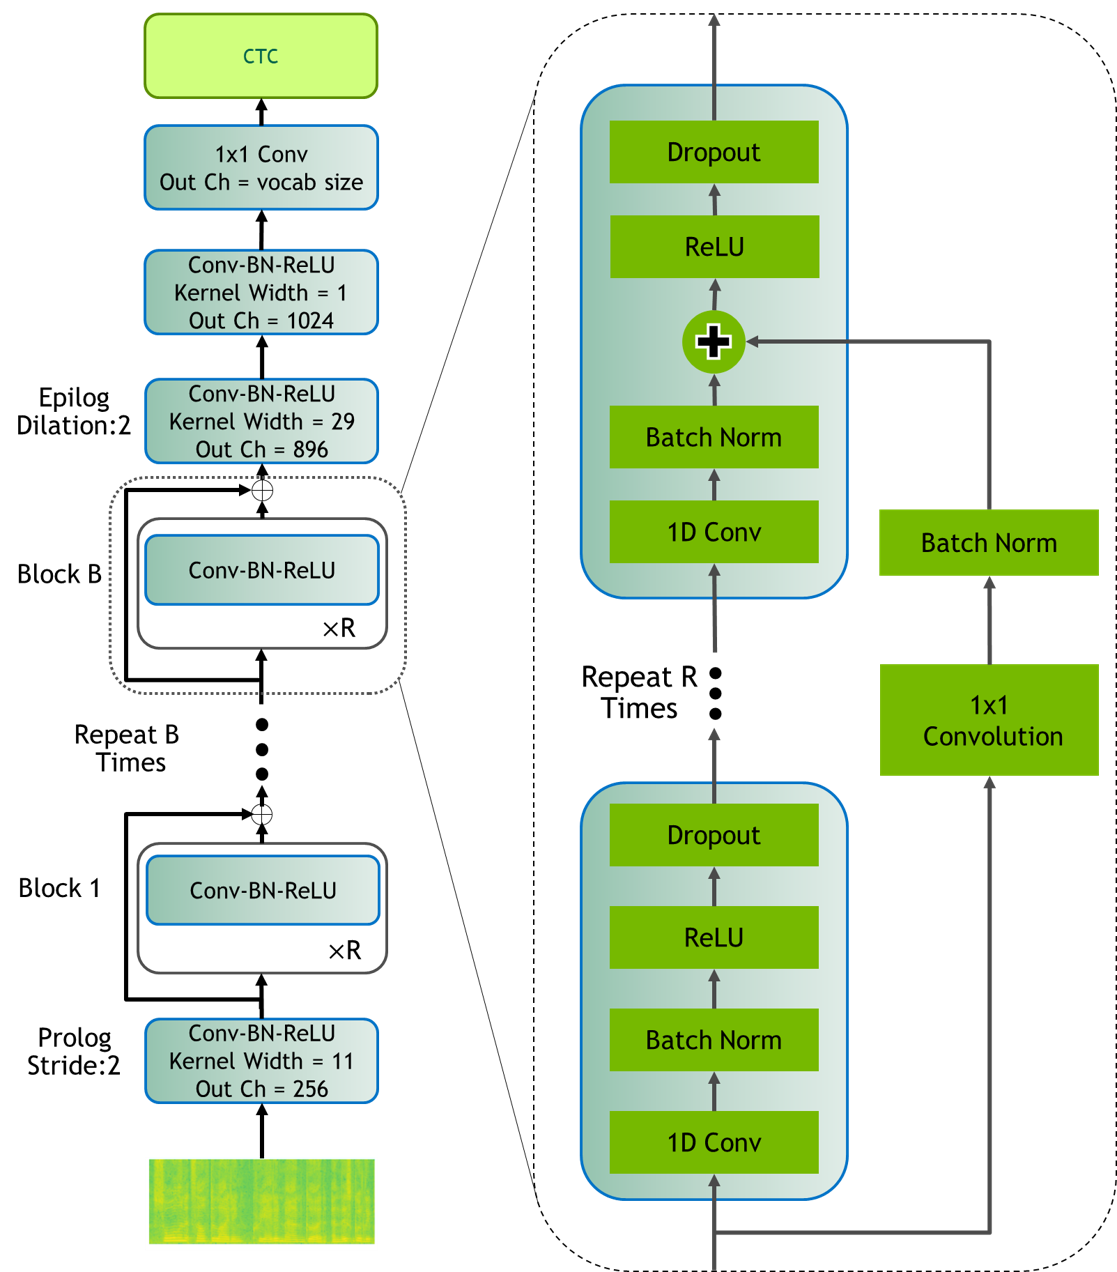
\includegraphics[width=0.5\linewidth]{figures/jasper_vertical.png}
    \caption{Block diagram of the Jasper architecture. Copied from Li et al.~\cite{li_jasper_2019}.}
    \label{fig:jasper}
\end{figure}

\subsection{QuartzNet}\label{sec:quartznet}
The QuartzNet architecture is based on Jasper with some key modifications, namely, that the one dimensional convolutions are replaced with ``one
dimensional time-channel separable convolutions'', as shown in Figure \ref{fig:quartznet}. As with Jasper, QuartzNet models are denoted as
\textit{QuartzNet $B\mbox{x}R$} with $B$ and $R$ representing the number of blocks and sub-blocks, respectively. However, blocks are repeated $S$
times and have a certain number of input and output channels, $c_{in}$ and $c_{out}$, respectively. Time-channel separable convolutions are separated
into two components: (1) convolutional layers that operate on each audio channel independently across time frames and (2) convolutional layers that
operate on time frames independently across all audio channels \cite{kriman_quartznet_2020}.

In Kriman et al.~\cite{kriman_quartznet_2020} experiments with QuartzNet were conducted on the LibriSpeech and Wall Street Journal speech corpora and
achieved near state-of-the-art performance on both. A transfer learning experiment was also performed (transferring between corpora). The model was
initially trained on LibriSpeech and Mozilla Common Voice, then fine-tuned on the Wall Street Journal corpus and also achieved near state-of-the-art
results \cite{kriman_quartznet_2020}. These results suggest that the QuartzNet architecture not only performs well on in-domain tasks, but can
generalize and fine-tune well on related data.

\begin{figure}
    \centering
    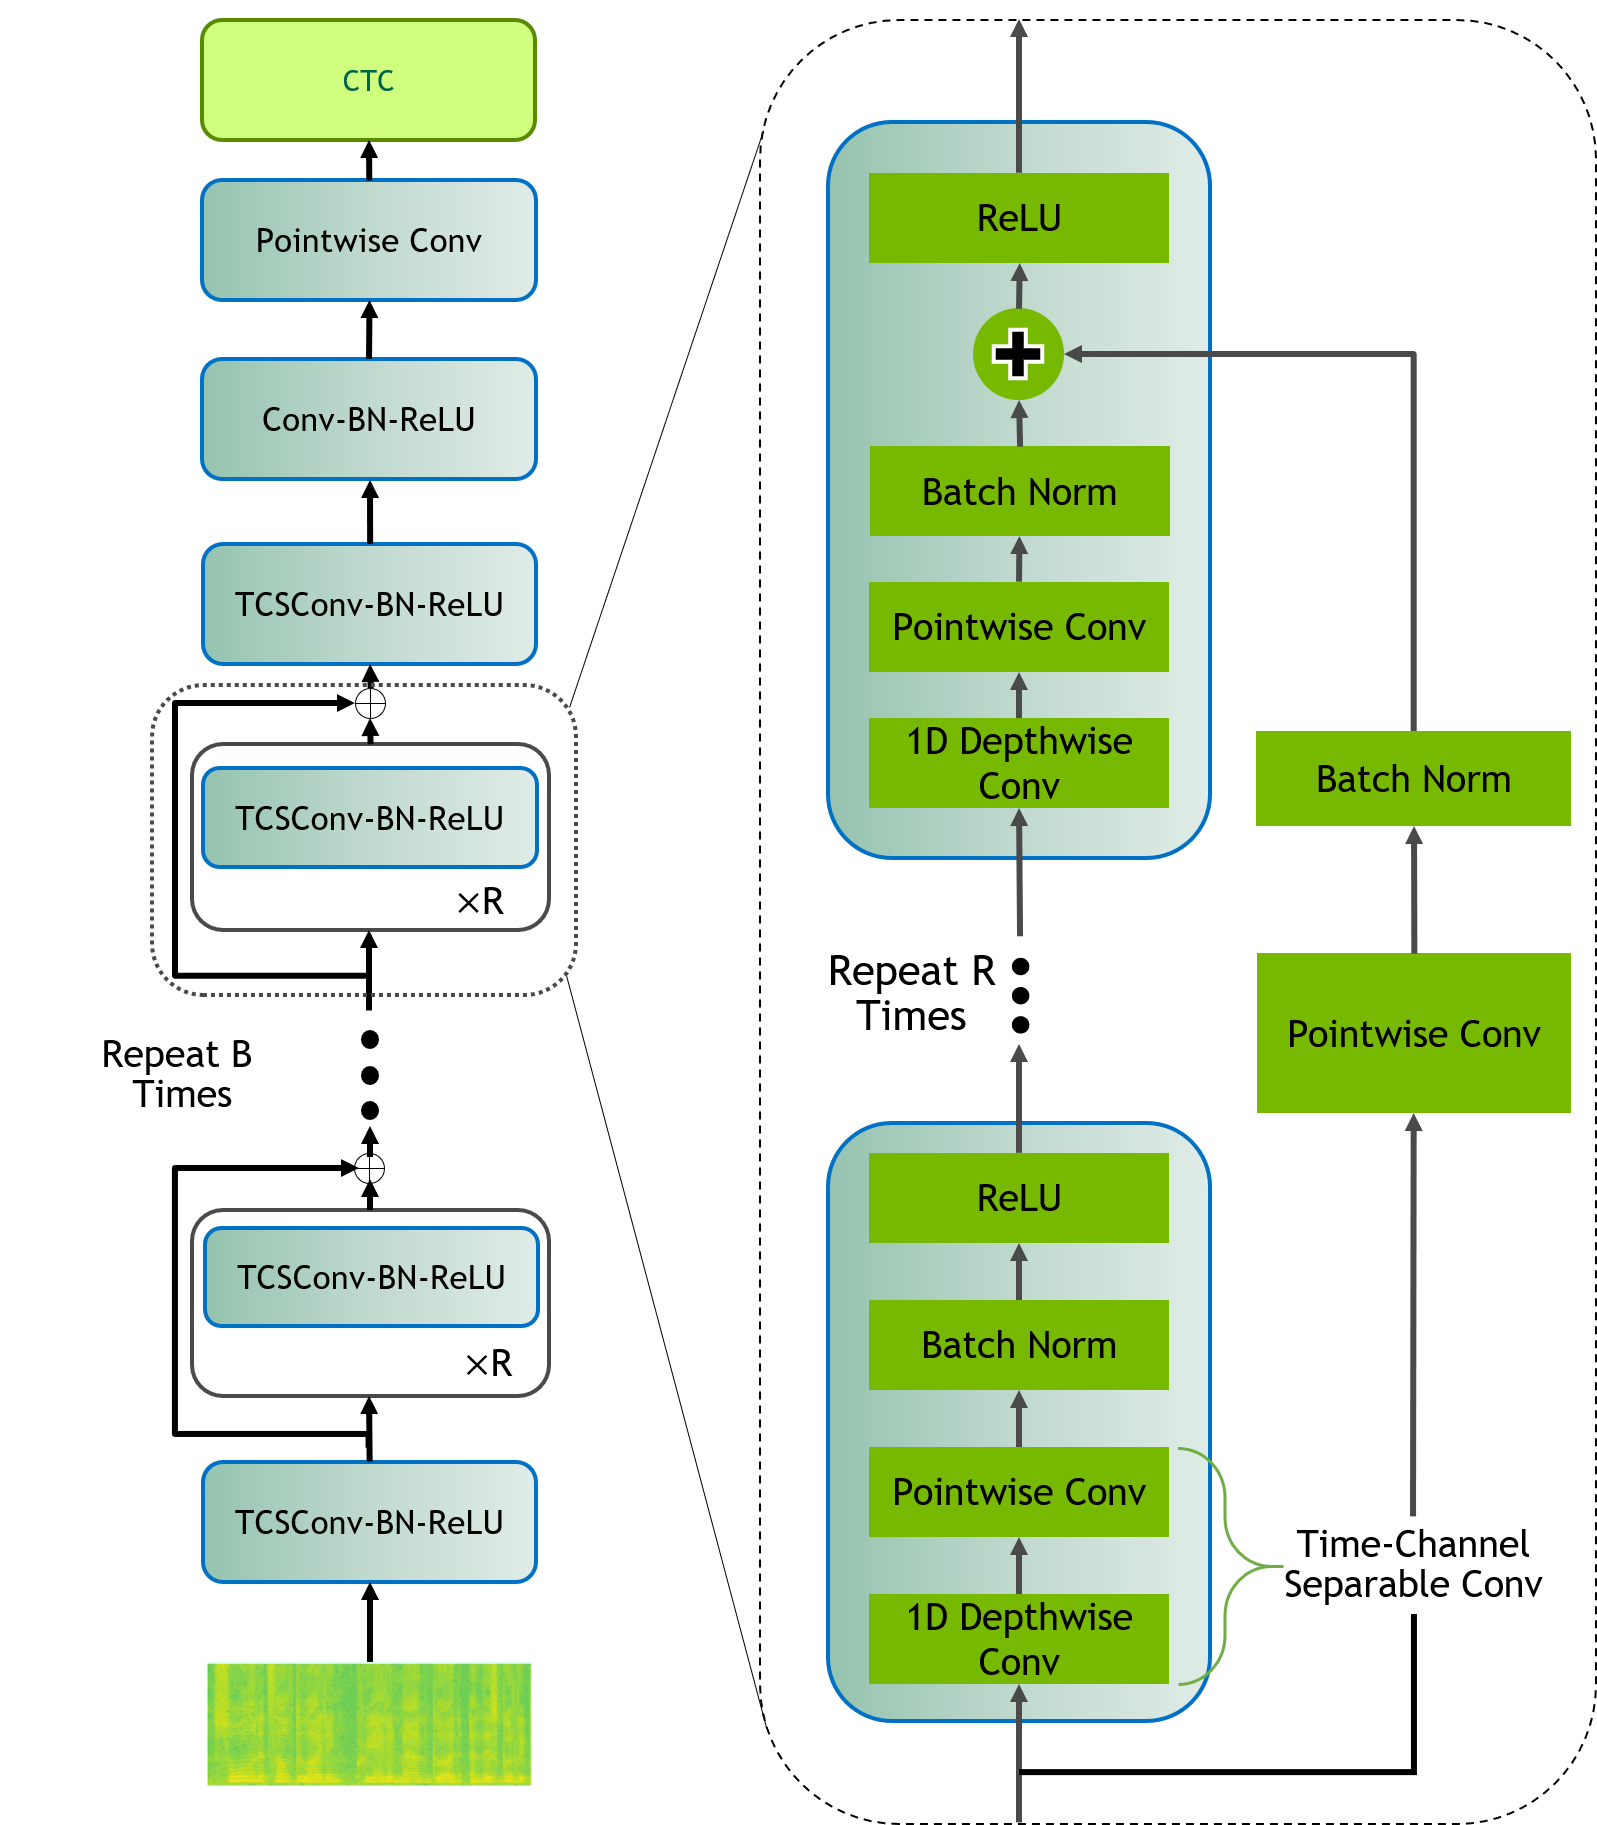
\includegraphics[width=0.5\linewidth]{figures/quartz_vertical.png}
    \caption{Block diagram of the QuartzNet architecture. Copied from Kriman et al.~\cite{kriman_quartznet_2020}.}
    \label{fig:quartznet}
\end{figure}

\subsection{Experiment Results}
This section will summarize the experiment setup, evaluation metrics, and final results of the two best performing ASR models. Two Jasper models with 10
blocks and 5 sub-blocks and two QuartzNet models with 15 blocks and 5 sub-blocks were trained from scratch and fine-tuned from pretrained
checkpoints; four models were evaluated in total. Each model used a vocabulary of 28 tokens; the English alphabet, an apostrophe, and a blank label.

\subsubsection{Performance Metrics}\label{sec:asr_performance_metrics}
% word error rate
This section defines the metrics used to track the performance of the ASR models during training and the performance of the models on the test
partitions of their datasets.

\textbf{Word Error Rate (WER)}. This is, simply, the number of words predicted incorrectly by the model. WER is based on the edit distance between the
models prediction and the prediction target \cite{hunt_figures_1990}. Let $N$, $S$, $I$, and $D$ be the number of words, substitutions, insertions,
and deletions, respectively. Then the WER is calculated as

\begin{equation}\label{eq:word_error_rate}
    \mbox{WER} = \frac{S + D + I}{N} \times 100
\end{equation}

\noindent
In this case, we calculate WER as a percentage by multiplying by 100. Note that it is possible for the WER to be greater than 100\% if
$S + D + I > N$. This can occur, for example, if the model predicts more words than are actually present in the audio signal.

\subsubsection{Optimizer}\label{sec:asr_optimizer}
The NovoGrad optimizer \cite{ginsburg_stochastic_2019} is used with the parameters shown in Table \ref{tab:novograd_params}.

\begin{table}[!t]
    \centering
    \begin{tabular}{l r}
        \toprule
        Parameter     & Value              \\
        \midrule
        $\beta_1$     & $0.8$              \\
        $\beta_2$     & $0.5$              \\
        $\epsilon$    & $1 \times 10^{-8}$ \\
        Learning rate & $0.01$             \\
        Weight Decay  & $0.001$            \\
        \bottomrule
    \end{tabular}
    \caption{NovoGrad optimizer parameters for the Jasper and QuartzNet ASR model training procedures.}
    \label{tab:novograd_params}
\end{table}

The Jasper model trained from scratch performed best overall with about a 15\% WER on the test data. The pretrained QuartzNet model that was
fine-tuned on the aggregated data performed second best among the evaluated models reaching a WER of about 30\%. The best-performing ASR models are
summarized in Table \ref{tab:asr_performance}. These tests were run using a greedy decoding method, meaning that at each time step, the most active
neuron i.e., that with the highest value after softmax was chosen as the prediction. These results can likely be improved further by adjusting the
parameters of the model. However we believe the most significant boost in performance can be achieved using a well-performing language model with a
beam search decoding algorithm. Beam search-based decoding methods use a language model and a beam search algorithm to determine predictions at each
time step. The most commonly used language model for these types of decoding methods is an N-gram and is what PyTorch's
\lstinline|CTCDecoder|\footnote{More specifically, the \lstinline|torchaudio| package of PyTorch.} \cite{paszke_pytorch_2019} and NeMo's
\lstinline|BeamSearchDecoderWithLM| \cite{kuchaiev_nemo_2019} use to decode predictions. The purpose of language models in beam search decoding
algorithms is to estimate the likelihood of the decoded sequence occurring based on the language models' knowledge of sequence structures. The beam
search algorithm is then used to select tokens to maximize the likelihood of the
sequence occurring. N-grams are left-associative language models (see Section \ref{sec:ngram}; assuming the model is being applied to the English
language in this case), which is an inherently limiting factor. A neural language model capable of representing sequences bidirectionally, such as
those covered in this work, is a significantly more robust method of language modeling in speech recognition and has been
used in the past to improve word error rates \cite{kriman_quartznet_2020,majumdar_citrinet_2021}. At least one instance of a deep learning-based
language model being used for beam search decoding in aviation applications. However, it did not perform well, likely due to the small size of the
dataset that it was trained on \cite{pellegrini_airbus_2019}. In the next section, the language model architectures, experiments, and results are defined
for the purpose of improving ASR model performance through the use of language models and downstream tasks such as callsign detection.

\begin{table}[!t]
    \centering
    \begin{tabular}{l r}
        \toprule
        Model                  & WER (\%) \\
        \midrule
        Jasper (scratch)       & 15.3     \\
        QuartzNet (pretrained) & 30.2     \\
        \bottomrule
    \end{tabular}
    \caption{WERs of the best-performing ASR models on the test partition of the corpus.}
    \label{tab:asr_performance}
\end{table}

\section{Language Models and Experiment Results}\label{sec:language_models}
This section introduces the chosen language model architectures and their pretrained checkpoints. Two transformer-based architectures, BERT and
RoBERTa, and one statistical/machine learning-based approach: N-gram language modeling.

The transformers are pre-trained using the same masked language modeling (MLM) objective presented in Devlin et al.~\cite{devlin_bert_2019} to train
BERT for bidirectional encoding representation and likewise in Liu et al.~\cite{liu_roberta_2019} for training RoBERTa. Given the results of the
RoBERTa pretraining and downstream task training thereafter, it was decided to eliminate the next sentence prediction (NSP) task that was used to
pretrain BERT. MLM and NSP pretraining are explained more in-depth in Section \ref{sec:bert} below.

\subsection{N-Gram}\label{sec:ngram}
An N-gram language model estimates the probability of a token occurring in a sequence based on the $N$ tokens preceding or succeeding that token.
In other words, for a sequence, $X$, of $T$ tokens

\begin{equation}\label{eq:ngram_sequence}
    X = \mbox{$w_1$, $w_2$, $w_3$, ..., $w_T$}\\
\end{equation}

\noindent
the probability of tokens occurring in order, in a sequence can be represented using the chain-rule of probability:

\begin{equation}
    \begin{gathered}
        P(X) = P(w_1) P(w_2|w_1) P(w_3|w_2, w_1) ... P(w_T|w_{T-1}, w_{T-2}, ..., w_1)\\
        P(X) = P(w_i)\prod_{i=2}^{T} P(w_i|w_{i-1}, w_{i-2}, ..., w_1)
    \end{gathered}
\end{equation}

\noindent
Except for the first token in the sequence, the probability of a token occurring at a specific point depends on the tokens preceding
it\footnote{The most common use case for an N-gram model is the preceding tokens.}. Due to this fact, N-grams are sometimes called left-associative
models (in a left-to-right language).

The probability of a token occurring at all is determined statistically as the number of occurrences in a corpus divided by the total number of tokens.

\begin{equation}\label{eq:ngram_prob_wj}
    P(w) = \frac{\phi_w(w)}{D_{tokens}}
\end{equation}

\noindent
where $P(w)$ is the probability of a token, $w$, occurring anywhere in the corpus, $\phi_w(w)$ is the number of times a specific token appears in the
corpus, and $D_{tokens}$ is the total number of tokens in the corpus, $D$. Computationally, determining the probabilities of the individual tokens in
the corpus is typically referred to as training or fitting the N-gram model.

$N$ is a predetermined value based on model or application requirements. While it can technically take any value from one to infinity, its usability
becomes very limited at the minimum sequence length in the corpus and unusable at any value at or above the maximum sequence length. Depending on
implementation, the time and resources required to train a model with a large value of $N$ can be very expensive. Common values for $N$ are one, two,
and three, sometimes called unigrams, bigrams, and trigrams, respectively.

\subsection{Transformer}\label{sec:transformer}
The transformer neural network uses an Encoder-Decoder architecture with multi-head self-attention layers throughout the network. Details of the
general design of the network will be laid out here in more detail, including the construction of the layers, sub-layers, and operation of the
attention mechanism. The design discussed here is identical to the network described in \textit{Attention Is All You Need}
\cite{vaswani_attention_2017} and is the base of the design of BERT and RoBERTa models discussed in Sections \ref{sec:bert} and \ref{sec:roberta},
respectively.

\textbf{The Encoder Stack}. The encoding layers (referred to as the ``Encoder Stack''; see Figure \ref{fig:transformer_encoder_stack}) are composed
of $N$ identical layers, each containing two sub-layers: (1) a multi-head self-attention mechanism and (2) a position-wise fully connected
feed-forward network. Each sub-layer includes a residual connection that is added to the output of the sub-layer and normalized. All sub-layers
produce outputs of dimension $d_{model}$. Vaswani et al.~\cite{vaswani_attention_2017} used $N=6$ encoding layers and $d_{model} = 512$ output
dimensions. The feed-forward network uses an inner dimension of $d_{ff} = 2048$

\begin{figure}
    \centering
    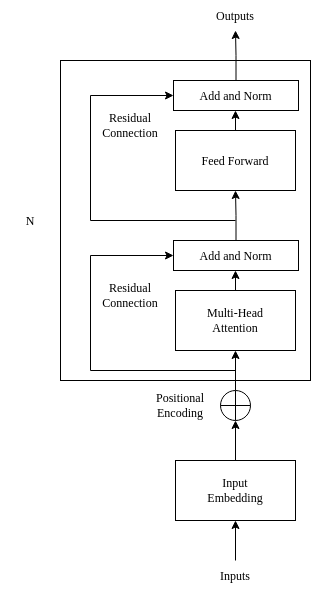
\includegraphics[width=0.5\linewidth]{figures/transformer_encoder_stack.png}
    \caption{The Encoder Stack of the transformer architecture. Modified from \cite{vaswani_attention_2017}.}
    \label{fig:transformer_encoder_stack}
\end{figure}

\textbf{The Decoder Stack}. The decoding layers are also comprised of $N$ layers (the ``Decoding Stack''; see Figure
\ref{fig:transformer_decoder_stack}) with three sub-layers for each layer: (1) a masked multi-head attention sub-layer, (2) a multi-head attention
sub-layer over the outputs of the Encoder Stack, and (3) a position-wise fully connected feed-forward network. The last two sub-layers are identical
to those in the Encoder Stack. Each sub-layer also includes a residual connection that is added to the output of the layer and normalized. The first
multi-head attention layer is modified to a masked multi-head attention layer, masking off tokens greater than the $i$th position. This, in
combination with the output embeddings being shifted right by one position, ensure that predictions for a token position, $i$, are only dependent on
outputs for positions less than $i$ \cite{vaswani_attention_2017}.

\begin{figure}
    \centering
    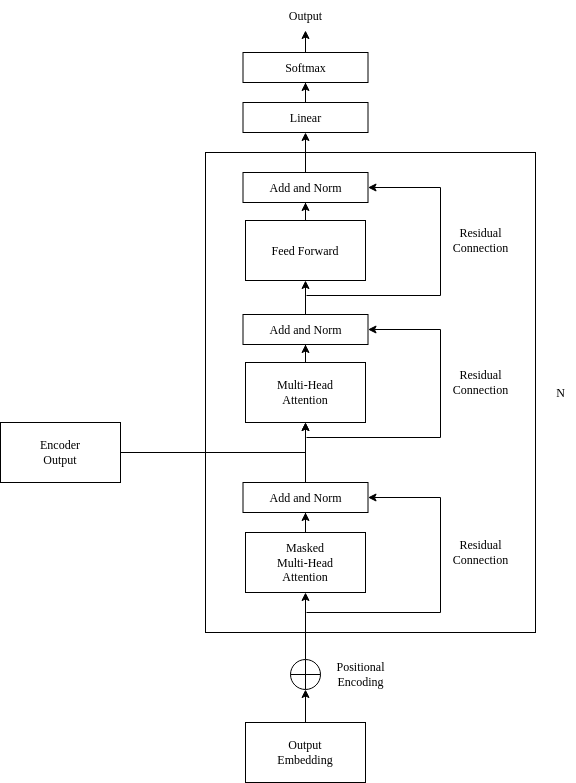
\includegraphics[width=0.6\linewidth]{figures/transformer_decoder_stack.png}
    \caption{The Decoder Stack of the transformer architecture. Modified from \cite{vaswani_attention_2017}.}
    \label{fig:transformer_decoder_stack}
\end{figure}

\textbf{The Multi-Head Attention Mechanism}. By the simplest of terms, attention mechanisms can be described as mapping a query and a set of keys and
values to an output. In the case of the transformer described by Vaswani et al.~\cite{vaswani_attention_2017}, a version of attention called ``Scaled
Dot-Product Attention'' is used. The query and keys are represented as vectors $Q$ and $K$, respectively, with dimensions of $d_k$. The values are
represented by a vector, $V$, with a dimension of $d_v$. A dot-product of the query and keys is computed, scaled by $\sqrt{d_k}$. A softmax function
is then applied to the output, given by equation (\ref{eq:softmax}).

\begin{equation}\label{eq:softmax}
    \mbox{softmax}(x) = \frac{\exp(x_i)}{\sum_{j=1}^{N}\exp(x_j)} \quad \forall i=1..N
\end{equation}

\noindent
Where $x$ is a vector of dimension $N$. Scaled-dot product attention can then be given by equation (\ref{eq:scaled_dot_attention}), below.

\begin{equation}\label{eq:scaled_dot_attention}
    \mbox{Attention}(Q,K,V) = \mbox{softmax}\left(\frac{QK^T}{\sqrt{d_k}}\right)V
\end{equation}

Multi-Head attention is defined as multiple scaled-dot product attention layers, running in parallel. More specifically, the queries, keys, and values
are linearly projected $h$ times with different learned linear projections to $d_k$, $d_k$, and $d_v$ dimensions, respectively. The attention function
is applied to each projection resulting in output vectors with dimensions of $d_v$. These are concatenated and linearly projected once more to produce
the output for the multi-head attention function \cite{vaswani_attention_2017}.

\begin{equation}\label{eq:multi_head_attention}
    \begin{gathered}
        \mbox{MultiHeadAttention}(Q,K,V) = \mbox{Concat}(\mbox{head$_1$, ..., head$_h$})W^O\\
        \mbox{where head$_i$ = Attention}(QW_i^Q, KW_i^K, VW_i^V)
    \end{gathered}
\end{equation}

\noindent
Where $W_i^Q$ and $W_i^K$ are weight matrices for the projections of dimensions $d_{model} \times d_k$, $W_i^V$ is a weight matrix for the projection
of dimension $d_{model} \times d_v$ and $W_i^O$ is a weight matrix for the projections of dimension $h d_v \times d_{model}$.

Vaswani et al.~\cite{vaswani_attention_2017} used $h = 8$ attention heads and $d_k = d_v = d_{model} / h = 64$.

\textbf{Token Embeddings}. Input and output tokens are converted to learned representations of dimension $d_{model}$ by the model
\cite{vaswani_attention_2017}.

\subsection{BERT}\label{sec:bert}
The purpose of BERT (Bidirectional Encoder Representations from Transformers) is to represent tokens in text sequences based on the tokens preceding
and following the token in question. Whereas an N-gram model represents token probabilities based on the $N$ tokens preceding a specific token or,
conversely, the $N$ tokens succeeding said token, BERT models can predict the probability of a token based on both preceding and succeeding tokens;
the bidirectionality novelty.

BERT is based on the transformer neural network described in Section \ref{sec:transformer} and uses an implementation that is nearly identical to that
of the original model \cite{devlin_bert_2019,vaswani_attention_2017}. The notable differences between the original implementation and the
implementation of the base and large BERT models are shown in Table \ref{tab:bert_params}.

\begin{table}
    \centering
    \begin{tabular}{l r r r}
        \toprule
        Model          & Layers ($N$) & Hidden Layer Size ($d_{ff}$) & Attention Heads ($h$) \\
        \midrule
        AIAYN          & 6            & 2048                         & 8                     \\
        BERT$_{base}$  & 12           & 768                          & 12                    \\
        BERT$_{large}$ & 24           & 1024                         & 16                    \\
        \bottomrule
    \end{tabular}
    \caption{Number of layers, hidden layer sizes, and number of attention heads for the base and large versions of the BERT model
        compared to the model used in \textit{Attention Is All You Need} (AIAYN) \cite{devlin_bert_2019,vaswani_attention_2017}.}
    \label{tab:bert_params}
\end{table}

\textbf{Representation of Inputs}. BERT uses a summation of the token embeddings (token IDs), segment embeddings (zero or one to represent the first
or second sentence in a sentence pair), and position embeddings (the index of the token in the sequence) to form model inputs. Additionally, the
WordPiece tokenizer algorithm (detailed in Section \ref{sec:wordpiece}) is used to segment tokens. The maximum sequence length of the model is 512
tokens and the size of the learned embeddings corresponds to $d_{model}$ (768 for BERT$_{base}$ and 1024 for BERT$_{large}$) \cite{devlin_bert_2019}.

\textbf{Masked Language Modeling}. The ability of BERT to represent text in a bidirectional context is achieved through the Masked Language Modeling
(MLM) pretraining task~\cite{devlin_bert_2019}. MLM pretraining chooses a certain percentage of token positions at random as labels for prediction;
those tokens are then replaced with either a ``mask'' token, a random token, or the original token according to preconfigured probabilities (BERT used
80\% for the mask token, 10\% for random tokens, and 10\% for the original/unchanged token). During training, the masked sequences are used as input
to the model, and the original is used as the prediction target. The model prediction is scored against the target using cross-entropy loss.

\textbf{Next Sentence Prediction}. While MLM conditions the model to represent tokens within sequences and predict the most probable token based on
its position in the sequence, NSP is meant to condition the model to understand relationships between sentences/sequences to support downstream tasks.
Since the BERT training set consists primarily of literary works and excerpts from Wikipedia, the model simply predicts whether two sentences appear
together (one after the other) in the original text, making this a binary classification task as opposed to MLM, which is a multi-class classification
task. Instead of a single sequence, the input consists of two sequences separated by a ``separation'' token and beginning with a ``classification''
token; these are represented by \lstinline|[SEP]| and \lstinline|[CLS]|, respectively in Devlin et al.~\cite{devlin_bert_2019}.

The special tokens specifying the beginning and end of input sequences are shared between tasks for symmetry between pretraining tasks. For both MLM
and NSP objectives, input sequences always start with a classification token and end with a separation token (see Figure
\ref{fig:bert_mlm_input_example}). Likewise, NSP inputs always begin with a classification token, and each input sequence is concatenated with a
separation token terminating each sequence (see Figure \ref{fig:bert_nsp_input_example} and equation (\ref{eq:bert_input_example})).

\begin{equation}\label{eq:bert_input_example}
    \begin{gathered}
        \mbox{[CLS], the, quick, brown, fox, [SEP]}\\
        \mbox{[CLS], the, quick, brown, fox, [SEP], jumps, over, the, [SEP]}
    \end{gathered}
\end{equation}

\begin{figure}
    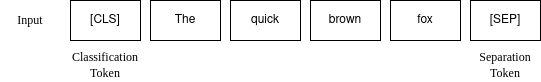
\includegraphics[width=\linewidth]{figures/BERT_MLM_input.png}
    \caption{An example of an input sequence for a masked language modeling pretraining task. Modified from Devlin et al.~\cite{devlin_bert_2019}.}
    \label{fig:bert_mlm_input_example}
\end{figure}

\begin{figure}
    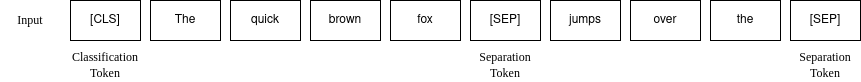
\includegraphics[width=\linewidth]{figures/BERT_NSP_input.png}
    \caption{An example of an input sequence for a next sentence prediction pretraining task.}
    \label{fig:bert_nsp_input_example}
\end{figure}

\subsection{RoBERTa}\label{sec:roberta}
As the name implies, the Robustly Optimized BERT Pretraining Approach (RoBERTa) is an iteration on BERT (described in Section \ref{sec:bert}, above).
The results from Liu et al.~\cite{liu_roberta_2019} indicate that BERT was initially significantly undertrained, so by training longer, with larger
batch sizes, on longer sequences, and dynamically changing the masking pattern applied to the MLM pretraining task, the performance of BERT was
improved. The new checkpoint of this version of BERT was, therefore, called RoBERTa. The architecture and parameters of the RoBERTa models are
identical to that of BERT.

The pretraining methodology introduced by RoBERTa eliminated the NSP pretraining task originally used in BERT and opted to increase the quantity of
training data along with the batch sizes and train the model longer. Lastly, there is a small difference in the construction of input sequences as
compared to BERT; input sequences always begin with a classification token (\lstinline|[CLS]|), and individual segments are separated by a separation
token (\lstinline|[SEP]|). Rather than having sequences end with a separation token, they are terminated with an end-of-sequence token
(\lstinline|[EOS]|). See equation (\ref{eq:roberta_input_example}) modified from Liu et al.~\cite{liu_roberta_2019}, below.

\begin{equation}\label{eq:roberta_input_example}
    \mbox{[CLS], $x_1$, $x_2$, ..., $x_N$, [SEP], $y_1$, $y_2$, ..., $y_M$, [EOS]}
\end{equation}

\subsection{Tokenization Algorithms}\label{sec:tokenizers}
% present and explain the tokenization algorithms used (possibly which models they correspond to)
Tokenization is the process of separating or segmenting words in sentences into their component ``tokens''. The tokenized version of a sentence is
referred to as a sequence. The rules by which the tokens are created or segmented depend entirely on the algorithm used. The simplest and most
intuitive way to do this is by creating tokens based on whitespace, i.e., each word in the corpus is treated as a token\footnote{The Huggingface
    Tokenizer library implements this as the \lstinline|WordLevel| tokenizer.}. While this is simple and works in theory, it does not consider that
not every word in a language will occur in a corpus. The inevitable possibility of a tokenizer seeing a word not in the original training corpus is
known as the out-of-vocabulary (OOV) problem~\cite{wu_googles_2016}. Several different algorithms have addressed the OOV problem. For brevity's sake,
only the tokenization algorithms used by the models in this thesis are defined and explained.

\subsubsection{WordLevel}\label{sec:wordlevel}
The WordLevel \cite{wolf_transformers_2020} tokenization algorithm, mentioned briefly as an introductory example above, is the most technically simple
algorithm among those introduced in this section. Tokens are extrapolated from words in a sentence based on the whitespace separating each word. This
means that contractions, hyphenations, etc. are treated as their own words, i.e.~ ``you'', ``you're'', and ``you've'' are all seen as unique, distinct
words tokenized and mapped to their integral representations.

An index of the words that appear in a corpus must be created to map individual tokens to numerical values or IDs. The numerical values for each token
are derived from this index. For the WordLevel algorithm, this process is referred to as the tokenizer model training (see Algorithm
\ref{alg:wordlevel_training}).

The first step of the training procedure is to index any specified special tokens, such as mask, classification, or separation tokens (this is why
special tokens often have low-valued token IDs). The second step is to split the sentences in the training data into individual words. This is done by
splitting each string based on whitespace; in other words, the tokenizer treats sentences as lists of words delimited by space characters. Lastly, the
tokenizer iterates through each word in each sentence, indexing new words as it finds them until all sentences in the training corpus have been
analyzed. Token IDs are then derived based on the word's position in the tokenizer index or vocabulary.

\begin{algorithm}[!t]
    \caption{Training procedure for the WordLevel tokenizer.}
    \label{alg:wordlevel_training}
    \begin{algorithmic}
        \State $D = \{s_1, s_2, ..., s_N\}$
        \Comment{$D$, $s_i$, and $N$ are corpus, sentence, and corpus length}
        \State $V \gets \{\varnothing\}$
        \Comment{$V$ is the tokenizer vocabulary and is initialized to the empty set}\\

        \For{$s \in D$}
        \State Split $s$ into words using whitespace as a delimiter such that
        \State $W=\{w_1, w_2, ... w_M\}$
        \Comment{$w$ and $M$ are words and sentence length}\\

        \For{$w \in W$}
        \If{$w \notin V$}
        \State $V \gets V;w$
        \Comment{Add $w$ to the vocabulary}
        \EndIf
        \EndFor
        \EndFor
    \end{algorithmic}
\end{algorithm}

Table \ref{tab:wordlevel_tokenization_example} shows the different representations of the input sentence over the course of the tokenization process.

\begin{table}[!t]
    \centering
    \begin{tabular}{l l}
        \toprule
        Tokenization stage & Representation                                                                            \\
        \midrule
        Input string:      & ``the quick brown fox jumps over the lazy dog''                                           \\
        Tokenized string:  & [``the'', ``quick'', ``brown'', ``fox'', ``jumps'', ``over'', ``the'', ``lazy'', ``dog''] \\
        Integral mapping:  & [5, 16, 9, 12, 13, 15, 5, 14, 11]                                                         \\
        \bottomrule
    \end{tabular}
    \caption{A simple example of the tokenization process of the WordLevel tokenization algorithm.}
    \label{tab:wordlevel_tokenization_example}
\end{table}

The algorithm's simplicity speaks for itself and serves as a good introduction to tokenization and an illustrative example of the OOV problem. Note
that the values of the integers representing the tokens are determined based on the order in which the tokens are seen during the training process
(special tokens are defined and, therefore, seen first), so these results are completely reproducible as long as the data appears in the same order.

The tokenization of words with shared roots but different suffixes is shown in Table \ref{tab:wordlevel_tokenization_shared_roots_example}. The
tokenizer sees all three words as independent and unique words since they are mapped to their own integer representations.

\begin{table}[!t]
    \centering
    \begin{tabular}{l l}
        \toprule
        Tokenization stage & Representation                    \\
        \midrule
        Input string:      & ``you you're you've''             \\
        Tokenized string:  & [``you'', ``you're'', ``you've''] \\
        Integral mapping:  & [18, 19, 20]                      \\
        \bottomrule
    \end{tabular}
    \caption{The results of tokenizing three words with the same roots and differing suffixes.}
    \label{tab:wordlevel_tokenization_shared_roots_example}
\end{table}

The tokenizer used to generate the examples in tables \ref{tab:wordlevel_tokenization_example} and
\ref{tab:wordlevel_tokenization_shared_roots_example} was trained on two sentences, notably lacking the word ``you'll''. Running the tokenizer on the
word ``you'll'' alone results in the output in Table \ref{tab:wordlevel_unk_word}. Although the word shares a root with some of the words in the
training data (``you'', ``you're'', and ``you've'') and is syntactically very similar, the tokenizer does not recognize the word at all (represented
by the ``[UNK]'' or unknown token). This word would be considered out-of-vocabulary since it did not appear in the training data and thus reveals one
of the major downsides of this algorithm, as mentioned in section \ref{sec:tokenizers}. This problem can be alleviated to some extent by modifying the
preprocessing strategy of the tokenizer to partition contracted words into their component parts, e.g.~the word ``you're'' would be partitioned to
\lstinline|[``you'', ``''', ``re'']|, however, it eventually reappears, for example, when using the past, present, and future tenses of a verb
(e.g.~``go'' and ``goes'' in the training data, then encountering the future tense: ``going'').

\begin{table}[!t]
    \centering
    \begin{tabular}{l l}
        \toprule
        Tokenization stage & Representation \\
        \midrule
        Input string:      & ``you'll''     \\
        Tokenized string:  & [``[UNK]'']    \\
        Integral mapping:  & [0]            \\
        \bottomrule
    \end{tabular}
    \caption{Results of running the WordLevel tokenizer on an unknown word similar to some of those in the training data.}
    \label{tab:wordlevel_unk_word}
\end{table}

\subsubsection{WordPiece}\label{sec:wordpiece}
% Wu et al. 2016; Schuster and Nakajima 2012
Schuster and Nakajima \cite{schuster_japanese_2012} developed the WordPiece algorithm as a word segmentation algorithm for language modeling in
Japanese and Korean voice search systems. It is further used by Wu et al.~\cite{wu_googles_2016} for neural machine translation tasks. The algorithm
demonstrated proficiency and increased performance for the models used in both tasks and effectively addresses the OOV problem.

One of the primary stipulations for this algorithm is effective and efficient handling of OOV words such that none are produced during normal
operation. To achieve this, during training, the vocabulary of the tokenizer is initialized to a basic set of characters; since WordPiece is designed
to be language agnostic, the initial vocabulary is specified as all basic unicode characters in addition to all ASCII characters.

The training procedure works by iterating over the vocabulary, combining two word units to maximize the likelihood over the training data, and
repeating until one of two stop conditions are reached:

\begin{enumerate}
    \item The predefined word limit is reached
    \item The increase in likelihood falls below the predefined threshold
\end{enumerate}

The training procedure is simple but computationally expensive. Schuster and Nakajima calculated the algorithm's time complexity at $O(K^2)$ where $K$
is the current size of the vocabulary~\cite{schuster_japanese_2012}. Due to the high time complexity of the algorithm, the authors suggest the
following considerations to reduce the computational complexity:

\begin{itemize}
    \item Test only pairs that actually exist in the training data
    \item Test only pairs with a significant chance of being best (high prior likelihood)
    \item Combine several clustering steps into a single iteration (for groups of pairs which don't affect each other)
    \item Only modify language model counts for the affected entries
\end{itemize}

Table \ref{tab:wordpiece_tokenization_example} shows an example of a WordPiece tokenizer model output on a sentence that was seen during the training
procedure (trained on the same data as the WordLevel tokenizer in Section \ref{sec:wordlevel}). Since this sentence was in the training data, the
segmentation is identical to that of the WordLevel tokenizer in Table \ref{tab:wordlevel_tokenization_example}, however, tokenization of similar
words (e.g.~words with shared roots or similar contractions) are handled differently, as in Table
\ref{tab:wordpiece_tokenization_shared_roots_example}. Since each word has a shared root word in the contractions (as well as an apostrophe separating
the contraction), the tokenizer segments each word and represents them as groups of small, more common tokens (thus with higher probabilities of
occurring). Additionally, the WordPiece algorithm effectively handles OOV words. For example, the OOV tokens in Table
\ref{tab:wordpiece_unk_word_similar}, with a shared root and similar contractions as those in Table
\ref{tab:wordpiece_tokenization_shared_roots_example}, which appear in the training data. The base of the contraction, ``you'', occurs in the training
data and the apostrophe in the contraction, so the tokenizer segments those parts of the word as tokens. The last part of the word, ``ll'', does not
appear at all in the training data, so it is broken down into its component characters, which are represented as ``l'' (beginning of a word) and
``\#\#l'' (segmented part of a word that should be concatenated to the previous token when they are recombined). Comparing this to the output of the
WordLevel tokenizer on the same word in Table \ref{tab:wordlevel_unk_word}, the WordPiece algorithm effectively addresses the OOV problem for words
similar to those in the training corpus and, according to the output of the WordPiece tokenizer in Table \ref{tab:wordpiece_unk_word}, for words
unlike those in the training corpus.

\begin{table}[!t]
    \centering
    \begin{tabular}{l l}
        \toprule
        Tokenization stage & Representation                                                                            \\
        \midrule
        Input string:      & ``the quick brown fox jumps over the lazy dog''                                           \\
        Tokenized string:  & [``the'', ``quick'', ``brown'', ``fox'', ``jumps'', ``over'', ``the'', ``lazy'', ``dog''] \\
        Integral mapping:  & [59, 98, 95, 88, 97, 91, 59, 90, 87]                                                      \\
        \bottomrule
    \end{tabular}
    \caption{A simple example of the tokenization process of the WordPiece algorithm.}
    \label{tab:wordpiece_tokenization_example}
\end{table}

\begin{table}[!t]
    \centering
    \begin{tabular}{l l}
        \toprule
        Tokenization stage & Representation                                            \\
        \midrule
        Input string:      & ``you you're you've''                                     \\
        Tokenized string:  & [``you'', ``you'', ``''', ``re'', ``you'', ``''', ``ve''] \\
        Integral mapping:  & [56, 56, 5, 71, 56, 5, 72]                                \\
        \bottomrule
    \end{tabular}
    \caption{Example of WordPiece tokenization of words with shared roots and differing suffixes.}
    \label{tab:wordpiece_tokenization_shared_roots_example}
\end{table}

\begin{table}[!t]
    \centering
    \begin{tabular}{l l}
        \toprule
        Tokenization stage & Representation                     \\
        \midrule
        Input string:      & ``you'll''                         \\
        Tokenized string:  & [``you'', ``''', ``l'', ``\#\#l''] \\
        Integral mapping:  & [56, 5, 17, 54]                    \\
        \bottomrule
    \end{tabular}
    \caption{WordPiece tokenization of an unknown word similar to some of those in the training data.}
    \label{tab:wordpiece_unk_word_similar}
\end{table}

\begin{table}[!t]
    \centering
    \begin{tabular}{l l}
        \toprule
        Tokenization stage & Representation                                                             \\
        \midrule
        Input string:      & ``anything''                                                               \\
        Tokenized string:  & [``an'', ``\#\#y'', ``\#\#t'', ``\#\#h'', ``\#\#i'', ``\#\#n'', ``\#\#g''] \\
        Integral mapping:  & [61, 49, 37, 53, 32, 36, 39]                                               \\
        \bottomrule
    \end{tabular}
    \caption{WordPiece tokenization of a word that does not appear in the training data and is not similar to any of the words in the tokenizer
        vocabulary.}
    \label{tab:wordpiece_unk_word}
\end{table}

\subsubsection{Byte-Pair Encoding}\label{sec:bpe}
% Sennrich et al. 2016; Gage 1994
The Byte-Pair Encoding (BPE) tokenizer algorithm was adapted from a data compression algorithm by Phillip Gage in 1994~\cite{gage_feb94_1994}. The data compression algorithm works by replacing common pairs of bytes in data with an unused byte to reduce the overall size of the data. The tokenization algorithm works under the same principle, merging frequent pairs of characters or tokens into one token~\cite{sennrich_neural_2016}.

The vocabulary of the tokenizer is initialized to the base set of characters (letters, numbers, punctuation, etc.~). The training procedure begins by counting all pairs (``A'', ``B'') of characters that appear in the training data and combines the most frequently occurring pair into one token (``A'', ``B'' $\rightarrow$ ``AB''). This process repeats until a specified vocabulary size has been reached (or a specified number of merge operations have occurred; the final vocabulary size is equal to the base character set plus the number of merge operations). Algorithm \ref{alg:bep_training} shows a minimal Python implementation for the BPE training procedure.

\begin{algorithm}[!t]
    \caption{BPE training algorithm implementation in Python. Modified from Sennrich et al.~\cite{sennrich_neural_2016}.}
    \label{alg:bep_training}
    \begin{lstlisting}[language=Python]
import re, collections

def get_stats(vocab):
    pairs = collections.defaultdict(int)
    for word, freq in vocab.items():
        symbols = word.split()
        for i in range(len(symbols)-1):
            pairs[symbols[i], symbols[i+1]] += freq
        return pairs
def merge_vocab(pair, v_in):
    v_out = {}
    bigram = re.escape(' '.join(pair))
    p = re.compile(r'(?<!\S)' + bigram + r'(?!\S)')
    for word in v_in:
        w_out = p.sub(''.join(pair), word)
        v_out[w_out] = v_in[word]
    return v_out

vocab = {...}
num_merges = 10
for i in range(num_merges):
    pairs = get_stats(vocab)
    best = max(pairs, key=pairs.get)
    vocab = merge_vocab(best, vocab)
    print(best)
    \end{lstlisting}
\end{algorithm}

Finally, comparing the BPE tokenization process with the WordLevel and WordPiece algorithms, we can see that the outputs of the algorithm are nearly
identical when the sentences being tokenized have words that appear in the training data (i.e.~the BPE outputs in tables
\ref{tab:bpe_tokenization_example} and \ref{tab:bpe_shared_roots_example} are almost identical to the WordPiece output in tables
\ref{tab:wordpiece_tokenization_example} and \ref{tab:wordpiece_tokenization_shared_roots_example} except the numerical representation of the tokens)
and very similar to that of the WordLevel tokenizer.

\begin{table}[!t]
    \centering
    \begin{tabular}{l l}
        \toprule
        Tokenization stage & Representation                                                                            \\
        \midrule
        Input string:      & ``the quick brown fox jumps over the lazy dog''                                           \\
        Tokenized string:  & [``the'', ``quick'', ``brown'', ``fox'', ``jumps'', ``over'', ``the'', ``lazy'', ``dog''] \\
        Integral mapping:  & [36, 70, 72, 66, 74, 69, 36, 68, 64]                                                      \\
        \bottomrule
    \end{tabular}
    \caption{The Byte-Pair Encoding tokenizer output for a string that appears in the training data.}
    \label{tab:bpe_tokenization_example}
\end{table}

\begin{table}[!t]
    \centering
    \begin{tabular}{l l}
        \toprule
        Tokenization stage & Representation                                            \\
        \midrule
        Input string:      & ``you you're you've''                                     \\
        Tokenized string:  & [``you'', ``you'', ``''', ``re'', ``you'', ``''', ``ve''] \\
        Integral mapping:  & [34, 34, 5, 33, 34, 5, 37]                                \\
        \bottomrule
    \end{tabular}
    \caption{Byte-Pair Encoding tokenizer output for syntactically similar words with shared roots.}
    \label{tab:bpe_shared_roots_example}
\end{table}

When testing the BPE algorithm on words that did not appear in the training data, it is clear that the BPE algorithm effectively deals with and
processes OOV words (tables \ref{tab:bpe_unk_similar} and \ref{tab:bpe_unk}), even when no subunits of the word appear in the training data (Table
\ref{tab:bpe_unk}).

\begin{table}[!t]
    \centering
    \begin{tabular}{l l}
        \toprule
        Tokenization stage & Representation                 \\
        \midrule
        Input string:      & ``you'll''                     \\
        Tokenized string:  & [``you'', ``''', ``l'', ``l''] \\
        Integral mapping:  & [34, 5, 17, 17]                \\
        \bottomrule
    \end{tabular}
    \caption{Byte-Pair Encoding tokenizer output for a word that did not appear in the training data, but is similar to some of the words in the
        training data.}
    \label{tab:bpe_unk_similar}
\end{table}

\begin{table}[!t]
    \centering
    \begin{tabular}{l l}
        \toprule
        Tokenization stage & Representation                                     \\
        \midrule
        Input string:      & ``anything''                                       \\
        Tokenized string:  & [``an'', ``y'', ``t'', ``h'', ``i'', ``n'', ``g''] \\
        Integral mapping:  & [39, 30, 25, 13, 14, 19, 12]                       \\
        \bottomrule
    \end{tabular}
    \caption{Byte-Pair Encoding tokenizer output for a word that did not appear in the training data and is not similar to any words in the training
        data.}
    \label{tab:bpe_unk}
\end{table}

\textbf{Byte-Level Byte-Pair Encoding}. This is a subset of the BPE algorithm that is also commonly used for NLP tasks such as neural machine
translation, language modeling, and generative tasks (GPT-2 uses a byte-level BPE tokenizer~\cite{radford_language_2019}). As Huggingface's
\lstinline|tokenizers| library implements it, this is a preprocessing step for the tokenizer model that maps all bytes in a string/sentence to
their own unique and visible character. Functionally, byte-level BPE is nearly identical to the standard BPE algorithm, described above, except that
the beginning of word symbol is rendered and represented by a visible character in the tokenized sequence (see Table
\ref{tab:byte_level_bpe_example}).

\begin{table}[!t]
    \centering
    \begin{tabular}{l l}
        \toprule
        Tokenization stage & Representation                                            \\
        \midrule
        Input string:      & ``anything''                                              \\
        Tokenized string:  & [``Ġa'', ``n'', ``y'', ``t'', ``h'', ``i'', ``n'', ``g''] \\
        Integral mapping:  & [36, 19, 30, 25, 13, 14, 19, 12]                          \\
        \bottomrule
    \end{tabular}
    \caption{Example of the output of a byte-level Byte-Pair Encoding tokenizer with the begging of a word represented with the ``Ġ'' character.}
    \label{tab:byte_level_bpe_example}
\end{table}

\subsection{Experiment Results}
This section will layout the experiment setup and results for the language modeling pretraining experiments. The language models are divided into two
categories, with two models in each category. The first category of models are those trained from scratch meaning that the models weights are
initialized according to a truncated normal distribution \cite{burkardt_truncated_2014}. The second category of models are based on pretrained
checkpoints from BERT and RoBERTa \cite{devlin_bert_2019,liu_roberta_2019}. Each category contains a BERT and RoBERTa model.

Considering the success of deep learning models with transformer-based architectures for language modeling and natural language processing (NLP)
tasks, more generally, in the conversational and written English domains, it follows that transformer architectures should see widespread use in
aviation English for domain-specific NLP tasks. However, the literature shows transformer-based language models have seen sparse use. The most notable
example of using a transformer neural network is the application of BERT for knowledge extraction from notice to airmen (NOTAM) messages
\cite{arnold_knowledge_2022}. While both BERT and RoBERTa have demonstrated that they perform well on English in general
\cite{devlin_bert_2019,liu_roberta_2019}, it is expected that the pretrained models will have limited performance due to the highly technical and
domain-specific nature of aviation English as well as the differing forms of the language; transcribed English speech as opposed to written English.
We expect the domain-specific terms and pronunciations will lead to a sufficiently different vocabulary from that of written English such that the
models trained from scratch will achieve better performance than the pretrained models.

A standard masked language modeling training procedure is used to pretrain the language models, as described in Section \ref{sec:bert}. Tokens are
masked at random as described in the MLM process in Section \ref{sec:bert}. Input sequences are padded to the maximum length the models accept with a
special \lstinline|[PAD]| token and truncated to the maximum length, if greater. The maximum sequence length for BERT and RoBERTa models is 512 tokens
\cite{devlin_bert_2019,liu_roberta_2019}. Based on the data analysis in Section \ref{sec:data_analysis}, there are few, if any, samples that meet or
exceed the maximum sequence length for BERT and RoBERTa models.

\subsubsection{Performance Metrics}\label{sec:performance_metrics}
The following metrics are defined and used to track the performance of the language models over the course of the training procedures. They also serve
as a means of measuring and comparing the performance of the models over the course of training and on the test partition of the corpus.

\textbf{Cross-Entropy Loss}. As mentioned previously, perplexity and cross-entropy loss (often shortened to loss) are used to track the model's
performance on the training and validation sets per epoch while training. Cross-entropy loss is defined below.

The cross-entropy loss between two probability distributions, $p$ and $q$, is typically defined as

\begin{equation}\label{eq:cross_entropy}
    H(p, q) = -\sum_{x \in X} p(x) \log q(x)
\end{equation}

\noindent
where $x$ is a single sample in the discrete distribution $X$. However, the way in which cross-entropy loss is measured can differ depending on
application. PyTorch \cite{paszke_pytorch_2019}, for example, defines and measures cross-entropy loss as follows:

Let $\mathcal{L}(x, y)$ be the cross-entropy loss function that outputs a $N \times 1$ vector, $L$, that contains the loss values for each sample in
a batch of $N$ samples.

\begin{equation}\label{eq:cross_entropy_defs}
    \mathcal{L}(x, y) = L = \{\mbox{$l_1$, $l_2$, ..., $l_N$}\}^T
\end{equation}

\noindent
Where $x$ is a $512 \times N$ vector representing model inputs (a sequence of tokens) and $y$ is a $1 \times N$ vector representing the target/label
for each sample in the batch. The cross-entropy loss for a single sample is then calculated as

\begin{equation}\label{eq:cross_entropy_loss}
    l_n = -\log \left[\frac{\exp(x_{n,y_n})}{\sum_{c=1}^{C}\exp(x_{n,c})}\right] \quad \forall n=1..N
\end{equation}

\noindent
where $l_n$ is the loss for an individual sample in the batch, and $C$ is the number of class labels. For language modeling, the set of class labels
is equivalent to the vocabulary of the tokenizer (and thus the language model). Numerical labels will correspond to token IDs. The loss for a batch is
calculated as the mean of the loss for each sample in the batch.

\begin{equation}\label{eq:cross_entropy_mean}
    \mathcal{L}(x, y) = \frac{1}{N}\sum_{i=1}^{N}l_i
\end{equation}

\noindent
Equation (\ref{eq:cross_entropy_mean}) can then be extended to find the mean cross-entropy loss over an epoch by swapping $l_i$ for batch means and
$\mathcal{L}(x, y)$ for the epoch mean. $N$ would then represent the number of batches in an epoch rather than the number of samples in a batch.

In this case, it is important to note that cross-entropy loss is, basically, a measure of the distance between a models prediction, $\hat{y}$, and the
intended target for the prediction, $y$.

\textbf{Perplexity}. This metric measures a model's ability to predict the most probable token in a sequence. It will measure and track how well the
language models can predict the most probable token for a specific point in a sequence. Perplexity is typically defined as

\begin{equation}\label{eq:ppl}
    \mbox{PPL} = 2^{-\frac{1}{N}\sum_{i=1}^{N} \log_2 q(x_i)}
\end{equation}

\noindent
where $N$ is the number of samples in a sequence, $x$ is an individual sample, and $q$ is the probability model (a language model, for the purposes of
this thesis). This is, essentially, the inverse of the probability of a sample appearing. A helpful way to view this is as how ``surprised'' a
probability model is to see a sample, thus the lower the probability of a sample, the higher the perplexity will be.

As with cross-entropy loss, the measure of perplexity can differ between implementations. PyTorch's \cite{paszke_pytorch_2019} implementation for
perplexity is defined as follows:

Let $P$ and $\hat{Y}$ be vectors representing the perplexity for samples in a batch and non-normalized output neurons in a neural network,
respectively.

\begin{equation}\label{eq:perplexity_defs}
    \begin{gathered}
        P = \{p_1, p_2, ..., p_N\}^T\\
        \hat{Y} = \{\hat{y}_1, \hat{y}_2, ..., \hat{y}_C\}^T
    \end{gathered}
\end{equation}

\noindent
Where $N$ is the number of samples in a batch and $C$ is the number of class labels. Then, the perplexity for each sample in a batch can be
calculated as

\begin{equation}\label{eq:perplexity}
    p_n = \exp \left[ \frac{1}{T}\sum_{i=1}^C - \log(\hat{y}_i) \right] \quad \forall n = 1..N
\end{equation}

\noindent
where $p_n$ is the perplexity for an individual sample in the batch, and $T$ is the number of tokens in the sample. The perplexity for the batch is
then calculated as the mean of the perplexities in the batch.

\begin{equation}\label{eq:perplexity_mean}
    \mbox{PPL} = \frac{1}{N}\sum_{i=1}^{N}p_i
\end{equation}

\noindent
Where $\mbox{PPL}$ is the mean perplexity over a batch with $N$ samples. This equation can then be extended to find the mean perplexity over each
batch in the epoch, swapping $p_i$ for batch means and $\mbox{PPL}$ for the epoch mean. $N$ would then represent the number of batches in an epoch
rather than the number of samples in the batch.

\subsubsection{Optimizer Settings}

The models are trained with the \textit{AdamW} optimizer \cite{loshchilov_decoupled_2019} using the hyperparameters in Table \ref{tab:optim_params}
based on the most effective pretraining configuration presented in \cite{devlin_bert_2019} and \cite{liu_roberta_2019}. These settings are kept
constant across language model pretraining experiments.

\begin{table}[!t]
    \centering
    \begin{tabular}{l r}
        \toprule
        Hyperparameter & Value              \\
        \midrule
        $\beta_1$      & $0.9$              \\
        $\beta_2$      & $0.98$             \\
        $\epsilon$     & $1 \times 10^{-6}$ \\
        Learning Rate  & $4 \times 10^{-5}$ \\
        Weight Decay   & $0.01$             \\
        \bottomrule
    \end{tabular}
    \caption{\textit{AdamW} hyperparameters for training BERT and RoBERTa models.}
    \label{tab:optim_params}
\end{table}

\subsubsection{Data Splits}
A train/test split of 70\% and 30\% and a validation split of 10\% of the training data was used for each model. A breakdown of the number of samples
in each split is shown in Table \ref{tab:corpus_splits}. The samples present in each split are kept consistent across language model experiments so
that the model performances are being compared based on identical data.

\begin{table}[!t]
    \centering
    \begin{tabular}{l r r}
        \toprule
        Corpus split & Split size (\%) & Samples \\
        \midrule
        Train        & 68.99           & 34,470  \\
        Validation   & 6.999           & 3,830   \\
        Test         & 30.01           & 16,415  \\
        \bottomrule
    \end{tabular}
    \caption{Number of samples and percentage of overall corpus by split.}
    \label{tab:corpus_splits}
\end{table}

\subsubsection{Results for the Models Trained from Scratch}\label{sec:scratch_pretraining_results}
The models trained from scratch were trained for 200 epochs. This value was found through two rounds of trial and error by monitoring the curves of
the loss and perplexity on the training and validation partitions of the corpus. This value was chosen to ensure that the pretraining procedure did
not have an overall negative effect on the model performance. Batch sizes of 16 were used over the course of training; this was the maximum batch size
that could be used with the hardware available\footnote{Values larger than 16 would sometimes cause Out of Memory errors on the GPU device used for
    training, so 16 was used to ensure all models trained continuously without error or interruption. Models were trained on a workstation with 64 GB
    of RAM and an NVIDIA RTX 3090 GPU with 24 GB of VRAM.}.

A graph of the average loss per step of scratch models on the training partition are shown in Figure \ref{fig:scratch_training_loss}. Both models
quickly converged to low loss values and maintained a relatively stable loss curve for the duration of the training procedure. This suggests that the
models are converging on either local or global minima.

\begin{figure}[!t]
    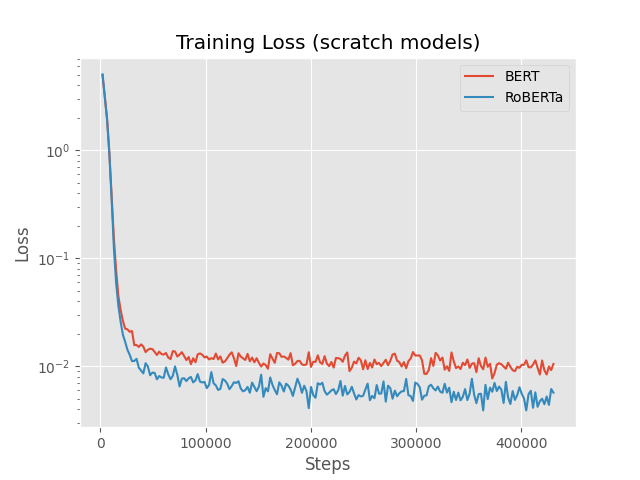
\includegraphics[width=\linewidth]{figures/scratch_training_loss.png}
    \caption{Cross-entropy loss of the models trained from scratch on the training partition of the corpus over time (steps).}
    \label{fig:scratch_training_loss}
\end{figure}

The graph of the perplexity of the models on the training partition of the corpus is shown in Figure \ref{fig:scratch_training_ppl}. The perplexity
of the models over time is erratic and rarely settles to a consistent trend over the duration of the training procedure. Also note that the perplexity
of the models is quite high throughout the training process. This is likely due to an issue with the models rapidly overfitting to the training data
as evidenced by graphs of the loss and perplexity of the models on the validation partition of the corpus in Figures \ref{fig:scratch_validation_loss}
and \ref{fig:scratch_validation_ppl}. This problem of rapid overfitting and consistently high perplexity is present in the results of the pretrained
models as well (see Section \ref{sec:pretrained_pretraining_results}). Theories as to why the models' perplexities are so consistently high and why
the models are overfitting so quickly will be explored in Section \ref{sec:results_comparison}.

\begin{figure}[!t]
    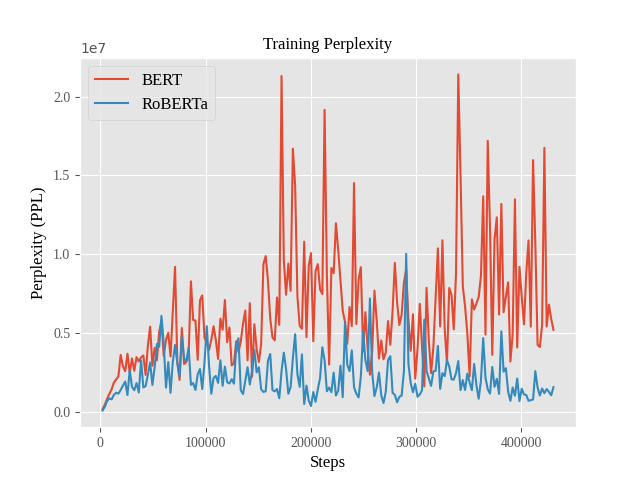
\includegraphics[width=\linewidth]{figures/scratch_training_ppl.png}
    \caption{Perplexity of the models trained from scratch on the training partition of the corpus over time (steps).}
    \label{fig:scratch_training_ppl}
\end{figure}

\begin{figure}[!t]
    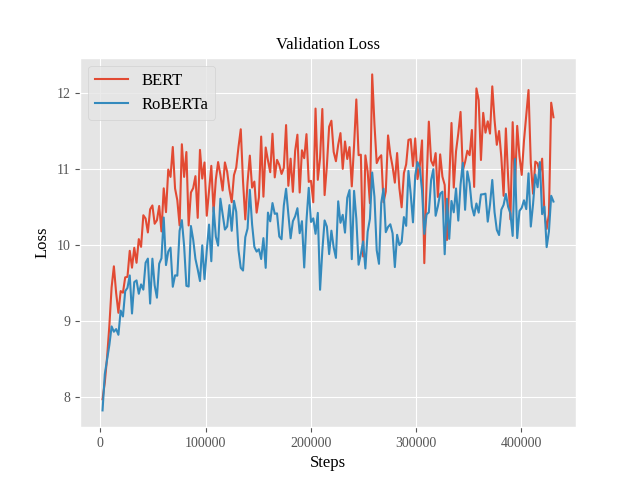
\includegraphics[width=\linewidth]{figures/scratch_validation_loss.png}
    \caption{Cross-entropy loss of the models trained from scratch on the validation partition of the corpus over time (steps).}
    \label{fig:scratch_validation_loss}
\end{figure}

\begin{figure}[!t]
    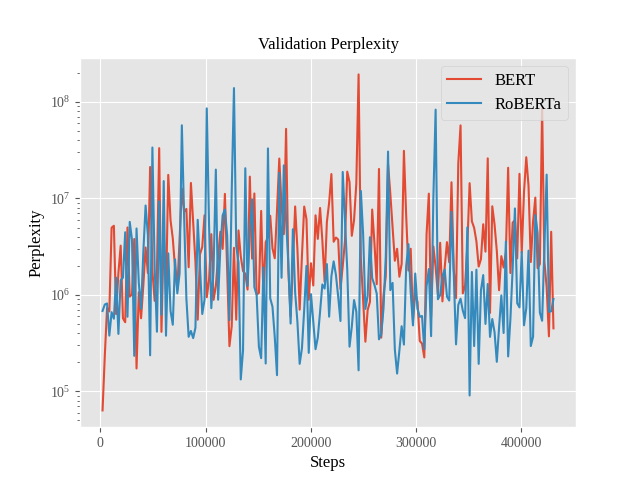
\includegraphics[width=\linewidth]{figures/scratch_validation_ppl.png}
    \caption{Perplexity of the models trained from scratch on the validation partition of the corpus over time (steps).}
    \label{fig:scratch_validation_ppl}
\end{figure}

\subsubsection{Results for the Pretrained Models}\label{sec:pretrained_pretraining_results}
The pretrained models were each trained for 100 epochs. As with the models trained from scratch, this value was found through two rounds of trial and
error by monitoring the loss and perplexity values of the models on the training and validation partitions of the corpus to find a value that would
ensure (or at least minimize) the net negative effects of overfitting. The batch size used for during training for the pretrained models is also 16
(for the same reason as with the models trained from scratch).

\begin{figure}[!t]
    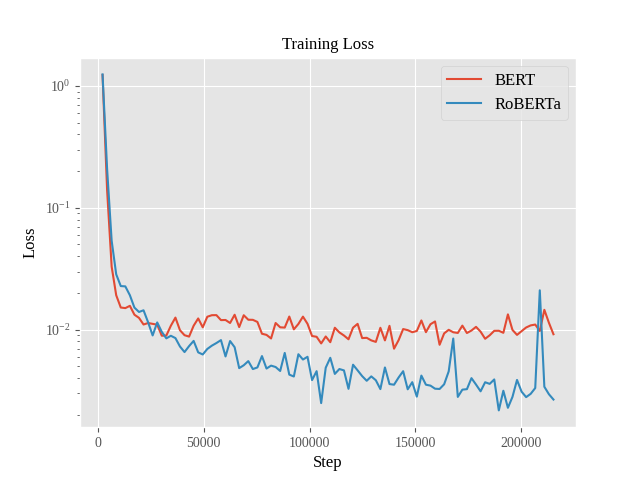
\includegraphics[width=\linewidth]{figures/pretrained_training_loss.png}
    \caption{Cross-entropy loss of the pretrained models on the training partition of the corpus over time (steps).}
    \label{fig:pretrained_training_loss}
\end{figure}

The graph of the training loss over time for the pretrained models can be seen in Figure \ref{fig:pretrained_training_loss}. Similarly to the models
trained from scratch, the pretrained models quickly converge to a consistent low loss value over the duration of the training procedure with little
to no deviation. The perplexity of the pretrained models on the training partition over the course of training, however, is much more stable and
exhibits a somewhat consistent trend. There are still large spikes in the value of the perplexity throughout the training procedure and the overall
values of the perplexity per step are still extremely high (note the scale of $10^9$ on the y-axis). As mentioned in Section
\ref{sec:scratch_pretraining_results}, this is likely due to overfitting of the models to the data, evidenced by the rapid overfitting shown in
Figures \ref{fig:pretrained_validation_loss} and \ref{fig:pretrained_validation_ppl}. A potential explanation as to why this phenomenon occurs is
proposed and explored in Section \ref{sec:results_comparison}.

\begin{figure}[!t]
    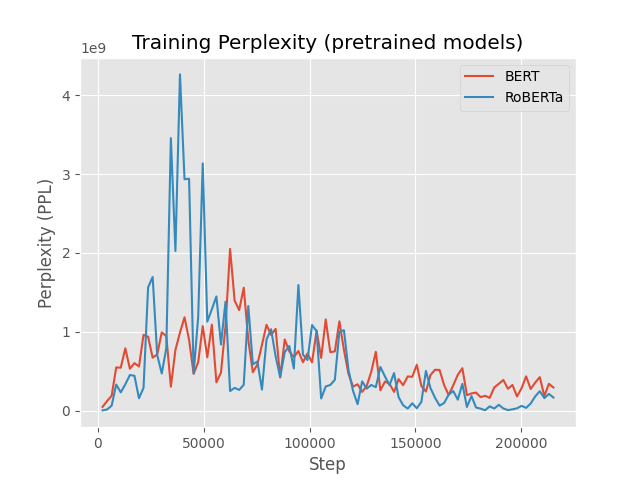
\includegraphics[width=\linewidth]{figures/pretrained_training_ppl.png}
    \caption{Perplexity of the pretrained models on the training partition of the corpus over time (steps).}
    \label{fig:pretrained_training_ppl}
\end{figure}

\begin{figure}[!t]
    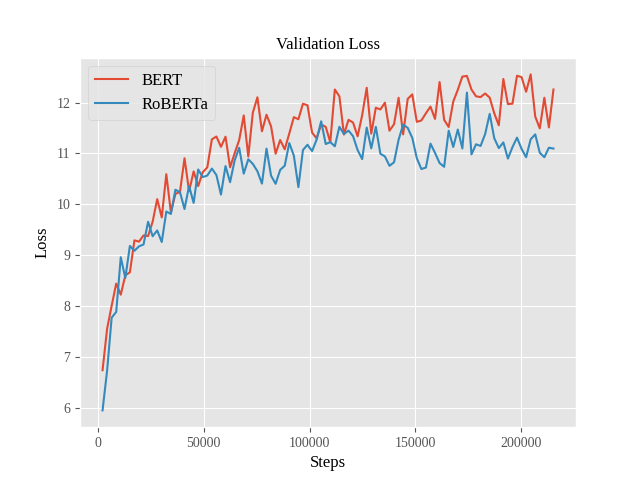
\includegraphics[width=\linewidth]{figures/pretrained_validation_loss.png}
    \caption{Cross-entropy loss of the pretrained models on the validation partition of the corpus over time (steps).}
    \label{fig:pretrained_validation_loss}
\end{figure}

\begin{figure}[!t]
    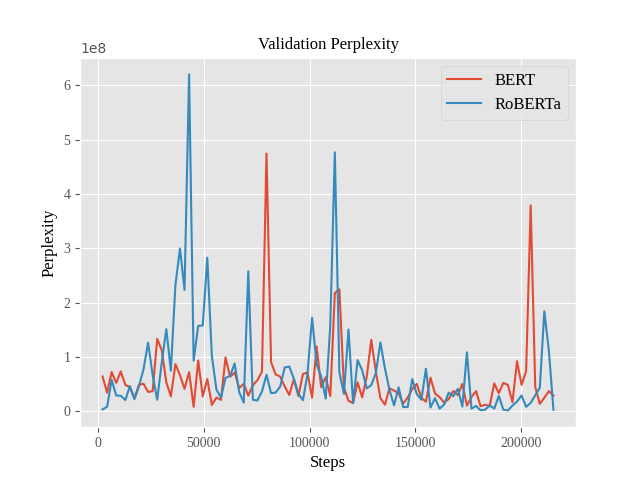
\includegraphics[width=\linewidth]{figures/pretrained_validation_ppl.png}
    \caption{Perplexity of the pretrained models on the validation partition of the corpus over time (steps).}
    \label{fig:pretrained_validation_ppl}
\end{figure}

\subsubsection{Comparison of Results}\label{sec:results_comparison}
Both classes of models (scratch and pretrained) quickly reach a steady state in terms of loss on the training partition of the corpus, although the
initial loss values are considerably different. Notably, the pretrained models start with a considerably lower loss, about 1.3, compared to the
models trained from scratch, which began with a loss value of just over 5.0. This indicates that the models are training well and starting to converge
on local or global minima. Although, as the graphs of the loss on the validation partition show, the models are quickly overfitting to the training
data, causing the models to begin performing poorly the validation data, which is not seen by the model during training.

Based on the trends exhibited by the cross-entropy loss of the models on the training and validation data, we would expect to see similar trends with
the perplexity on the training and validation partitions. However, the perplexity of the models on the training and validation data yields interesting
and somewhat unexpected results. Although the pretrained models have a more stable curve over time, the models trained from scratch result in a
lower perplexity. The final perplexity values (over the training set) of the models trained from scratch were markedly better than that
of the pretrained models. At the end of training, the BERT and RoBERTa models trained from scratch had perplexity values of $0.52\times 10^7$ and
$0.16\times 10^7$, respectively, whereas the pretrained models reached perplexity values of $0.29\times 10^9$ and $0.17\times 10^9$, for BERT and
RoBERTa, respectively. Using the following equation

\begin{equation}\label{eq:relative_difference}
    \mbox{RD} = \frac{v - v_{ref}}{v_{ref}}
\end{equation}

\noindent
where $v$ is a tested value and $v_{ref}$ is a reference value. The relative difference in perplexity between the scratch and pretrained models on the
final training epoch is 55.24 for the BERT models, and 104.57, for the RoBERTa models. Using the following equation for absolute difference,

\begin{equation}\label{eq:absolute_difference}
    \mbox{AD} = |a - b|
\end{equation}

\noindent
this equates to an absolute difference of $28.74 \times 10^7$ and $16.43 \times 10^7$ for the BERT and RoBERTa models, respectively.

The results from the training procedure show that the models trained from scratch outperformed their pretrained counterparts. This initially indicates
that pretraining models on in-domain data may achieve the best language model performance, then continuing to fine-tune on specific downstream tasks.
This seems to be a direct contradiction of the current recommended practice of using one of the pretrained checkpoints from Devlin et
al.~\cite{devlin_bert_2019} and Liu et al.~\cite{liu_roberta_2019} then fine-tuning on specific downstream tasks. However, this is only partially
upheld by the results of the model performance on the test partition of the corpus (Table \ref{tab:pretraining_results}). For the BERT models, the
pattern exhibited during training is consistent with the results on the test partition, resulting in a relative difference of 8.62 and an absolute
difference of $1.24 \times 10^7$ (using equations (\ref{eq:absolute_difference}) and (\ref{eq:relative_difference}), respectively). For the RoBERTa
models, however, the relative difference in perplexity is -0.34 with an absolute difference of $0.36 \times 10^7$. These results show that the
pretrained RoBERTa model performed better during pretraining than the corresponding model that was trained from scratch, unlike the BERT models. The
loss of each model over the test set is somewhat high, but they are around the same values for each model, which is consistent with the loss
statistics during training. A higher loss value on unseen (test) data is expected.

The BERT model trained from scratch had the best performance among the tested models followed closely by the pretrained RoBERTa model. The pretrained
BERT model used both MLM and NSP pretraining objectives to create the checkpoint used in this thesis. The pretrained RoBERTa model, on the other hand,
used only the MLM pretraining objective. It is readily apparent from the results of \cite{liu_roberta_2019} that RoBERTa's modified pretraining
methodology resulted in better model performance for in-domain problems. However, it seems that the pretraining method also allows RoBERTa to
generalize better than BERT when transfer learned to other NLP domains. It is conceivable that, given additional training data in the future, the
pretrained RoBERTa model could surpass the performance of the BERT model trained from scratch. However, with the current volume of data available in
this domain, it is clear from the models' results on the corpus test partition that a BERT model trained from scratch will still be the best option
for aviation English NLP tasks.

\begin{table}[!t]
    \centering
    \begin{tabular}{l r r}
        \toprule
        Model                & Loss  & Perplexity ($\times 10^7$) \\
        \midrule
        BERT (scratch)       & 10.54 & 0.14                       \\ % 1435064.875
        RoBERTa (scratch)    & 11.41 & 1.04                       \\ % 10376598.000
        BERT (pretrained)    & 11.00 & 1.38                       \\ % 13805354.000
        RoBERTa (pretrained) & 11.80 & 0.68                       \\ % 6816011.500
        \bottomrule
    \end{tabular}
    \caption{Results on the test set of data after pretraining the BERT and RoBERTa models from scratch and pretrained checkpoints. Loss and
        perplexity values are averaged over the test partition of the corpus. For both perplexity and loss; lower values are better.}
    \label{tab:pretraining_results}
\end{table}

With the results and performance of the models established relative to each other, the high perplexity of each model must be addressed. While the loss
values converge nicely during training, the perplexity is somewhat erratic and consistently high, rarely converging to a consistent curve. However, it
exhibits a clear trend as training progresses. Adjusting the hyperparameters of the optimizer did not solve this issue, and changing the
hyperparameters of the model (e.g.~sequence length, number of hidden layers, attention heads, etc.~) was not desirable for performing a direct
comparison between the pretrained checkpoints and the base models to study the effectiveness of the models on orthographic transcriptions of aviation
English. The validation curves for each model (Figures \ref{fig:scratch_validation_loss} and \ref{fig:pretrained_validation_loss}) clearly suggest
that the language models are rapidly overfitting to the training data, which is what is causing the loss on the validation partition to increase as
the models are trained further. It is difficult to determine what exactly is causing this phenomenon of the models rapidly and extremely overfitting
to the training data, so several theories were developed in an attempt to explain it (some of which will be elaborated upon in Section
\ref{sec:future_work}):

\textbf{Small volume of training data}. Especially when compared to \textit{Attention is All You Need}, BERT, and RoBERTa,
\cite{vaswani_attention_2017,devlin_bert_2019,liu_roberta_2019} the number of samples used in the training data dwarfs that of the state-of-the-art.
It has been exhaustively demonstrated that neural networks perform better with large volumes of data. The inception of RoBERTa itself is based on the
idea that BERT was not trained on enough data \cite{liu_roberta_2019}. Increasing the volume of in-domain data used for pretraining (and training)
would be the most effective way to immediately improve the performance of the models.

\textbf{Different forms of English}. The BERT and RoBERTa pretraining checkpoints were created by training the models on literary works and typed
articles such as those from \textit{Wikipedia}. The data used in this work are orthographic transcriptions of aviation English, and while the two data
sources share the common root of English, transfer learning from the casual style of written English to the technical, highly specific use of aviation
English yields limited results, as evidenced above, especially with relatively small amounts of data.

\textbf{Mixed regional data sources}. As described in Section \ref{sec:data_source}, the data aggregated for use here comes from several different
regions, namely international airports in the US \cite{godfrey_air_1994} and international and domestic airports in Europe
\cite{smidl_air_2019,hofbauer_atcosim_2008,szoke_detecting_2021}. During data processing, it was ensured that only English transcriptions were
included in the corpus. However, proper nouns from each region will be present in the data. Additionally, dialectical differences and varying levels
of English proficiency will affect the structure of token sequences across regions. All of these combined facets may contribute to the high perplexity
of the language models relative to other works. It should be noted that the varied regional data sources are not necessarily bad. Depending on the
application and desired robustness of the model, the ability to interpret international sources and contexts can be desirable for model selection;
however, it will require significantly more data and proportionally balanced regional contexts within the corpus for the pretraining process to be
effective for downstream tasks.

Up to this point, we have followed a procedure for studying the effectiveness of the models that is somewhat symmetrical to that of BERT and RoBERTa,
so at this point, the models should be trained for downstream tasks to measure the effectiveness of the pretraining procedures further. In the
aviation domain and for this particular data, that would mean training for tasks such as callsign identification, speaker identification, flight phase
classification, clearance recognition, etc. However, labels for these tasks are not present in the corpora used here. Corpora with relevant labels for
downstream tasks could not be obtained within an appropriate time to run and include the experiments in this work. Some potential algorithms were
developed to mine labels from the corpora aggregated for this work, which will be expanded upon in section \ref{sec:future_work}. For these reasons,
testing model performance and effectiveness on downstream tasks must be left for future work.

\section{Conclusions}\label{sec:conclusion}
Four aviation English corpora are aggregated and unified for use in neural language modeling and speech recognition. A masked language modeling
pretraining methodology is then used to pretrain two classes of BERT and RoBERTa language models (models trained from scratch and pretrained models
transfer learned to aviation English). For ASR we used MFCCs, calculated from the audio signals aggregated from the aviation English corpora, and the
transcripts used for language modeling to train and evaluate the models.

Contrary to the recommended best practice of using pretrained checkpoints and training for downstream tasks, we find that, in the domain of aviation
English, models achieve better performance when pretrained from scratch than model checkpoints transfer learned from the available BERT and RoBERTa
pretrained checkpoints. Although the pretrained RoBERTa model achieved better performance on the test partition of the corpus than expected, the
pretraining methods laid out in this thesis resulted in the BERT model trained from scratch achieving the lowest loss and perplexity overall. This
trend also emerges in the ASR models; the Jasper model trained from scratch achieved the best performance among the models evaluated, including those
from pre-existing checkpoints.

The results from the experiments in this work indicate that models trained from scratch for natural language processing tasks with limited data
availability in the aviation domain are more effective than transfer learning pretrained models. Thus, models trained from scratch should be
fine-tuned and used for downstream tasks over pretrained models. The most significant limiting factor to the performance of the models is the small
volume of aviation English data available for pretraining and downstream task use. Investment in creating expansive, high-quality, openly available
aviation English corpora with appropriate formatting for developing machine learning applications is also highly recommended.

Based on the results from training both ASR and language models from scratch and comparing the results with those fine-tuned from existing
checkpoints, it is clear that, in both cases, the models trained from scratch not only have better performance overall but will also have a higher
likelihood of reliable callsign detection/identification performance due to the higher individual performance overall. For future applications
of NLP tasks in the aviation English domain, we recommend pretraining models from their base initializations using in-domain data and fine-tuning on
additional labeled in-domain data for downstream tasks.

\section{Future Work}\label{sec:future_work}
This section is intended to serve as a brief proposal or set of suggestions for future work based on the results of this work. The main focus of these
suggestions is corpus-specific algorithms and data augmentation techniques to enable testing and experiments to determine the effectiveness of the
pretraining procedures covered earlier in this thesis.

\subsection{Next Sentence Prediction}
This training procedure was introduced by Devlin et al.~\cite{devlin_bert_2019} as a pretraining procedure for BERT and is described in more detail in
Section \ref{sec:bert}. This can be used on top of masked language modeling for language model pretraining. However, it requires a knowledge of which
sequences in the corpus appear next to each other. For pretraining transformer-based neural language models for the aviation domain (with orthographic
transcriptions), this same procedure can be used to classify whether two transmissions occur in the correct order. Generalizing a bit, we can consider
two individual transmissions to be $A$ and $B$; the training objective for the network is then to predict whether transmission $B$ occurs in response to
transmission $A$. This would be considered a binary classification task; $B$ either occurs in response to $A$ or it does not. In practice, for a true
label (meaning $B$ does, in fact, occur in response to $A$), transmission $A$, for example, can be a pilot request to ATC and transmission $B$ would
be ATC's response. A false label (meaning $B$ does not occur in response to $A$) would be made up of transmissions randomly shuffled such that $A$ and
$B$ do not occur together in the corpus. Note that, since these are only two transmissions, neither $A$ nor $B$ will necessarily be one side of the
transmission i.e.~$A$ can be either a pilot or ATC. Of the four corpora used in this work, ATCC is the only corpus that can be mined for an NSP-like
pretraining procedure since the raw transcripts have indicators for time (start and end indicators), transmitting party, and intended receiver. With
this information, we can estimate the correct order of transmissions between two parties to a reasonable degree of certainty (manually or
programmatically). For example, using the following transmissions from ATCC corpus, in which the Boston-Logan tower is communicating with PAA540. The
transmission below can be used as $A$:

\begin{quote}
    CLIPPER SIXTY FIVE FORTY IS AH FOUR FROM RIPIT CLEARED FOR THE I L S D M E TWO SEVEN APPROACH
\end{quote}

\noindent
and the response from PAA540 to the Boston-Logan tower can be used as $B$:

\begin{quote}
    AH ROGER CLEARED FOR THE APPROACH AH CLIPPER FIVE FORTY THANK YOU
\end{quote}

\noindent
In this case, $A$ and $B$ occur in the middle of an interaction. There are two transmissions between PAA540 and the Boston-Logan tower that occur prior
to the two above. We can consider the two instances of $A$ and $B$ above as a true label, meaning they occur one after the other in the corpus. To
construct a false label, we can simply reverse the input of $A$ and $B$, i.e.~$A$ becomes $B$ and $B$ becomes $A$, or choose another transmission at
random from the corpus to replace either $A$ or $B$. For proper construction of the corpus for the NSP pretraining task, the distribution of true and
false labels should be evenly balanced. If there are 500 samples labeled as true, then there should be 500 samples labeled as false.

\subsection{Callsign Detection/Identification}
This is the process of identifying an aircraft callsign from the transcription of the spoken callsign. This is a popular subtask for automatic speech
recognition applications in aviation, but postprocessing speech recognition outputs can also be accomplished through a language model. ATCC is a good
candidate corpus for this task. There are two potential methods for implementing this as a downstream task: (1) In transmissions from air-traffic
controllers to specific aircraft, use the receiver (the ``TO'' label in ATCC's raw transcriptions) as the label for each sequence or (2) Identify the
sequence of tokens, in each transmission, that correspond to the callsign of the aircraft and use those tokens as the labels for each sequence. Each
of these methods brings its problems. The first method effectively creates an ever-expanding classification problem with infinitely many labels, so a
tokenization or decoding scheme must be created to address this. The second method requires manually labeling every sequence in the corpus, which may
not be feasible in all cases. Lastly, both methods may lack sufficient context to predict aircraft callsigns correctly. Callsigns are agreed upon
between air carriers and air traffic control, but the callsign used will not always correspond directly to the air carrier's official three-letter
designation for flights. For example, United Airlines uses the three-letter designator ``UAL'', however, the agreed upon spoken, and therefore
transcribed, callsign is ``united'', so the flight ``UAL774'' will use the callsign ``united seven seven four''\footnote{The FAA maintains a list of
    companies, callsigns, and three-letter designators at \url{https://www.faa.gov/air_traffic/publications/atpubs/cnt_html/chap3_section_4.html}}.
General aviation (GA) callsigns introduce more variability and do not use previously agreed upon callsigns. Instead, for general aviation (GA)
aircraft, the spoken information is based on the registration or tail number of the aircraft, but not every element of the registration number is
necessarily required information in communications. For example, the FAA does not require the make or region of registration of the aircraft in spoken
communications, however, they can and do appear in communications. The following transcript is taken from ATCC and is a communication from ATC to an
aircraft with the registration number ``N01C'':

\begin{quote}
    TWIN CESSNA ZERO ONE CHARLIE TURN RIGHT HEADING ZERO NINER ZERO
\end{quote}

\noindent
Note that the make of the aircraft, though not required, is included and the region of registration (the \textit{N} at the beginning of the
registration number) is excluded. The callsign that should be identified in this case is ``TWIN CESSNA ZERO ONE CHARLIE'' and, ideally, this should
be mapped to the registration ``N01C'', although this is difficult without additional context such as the region of airport and make of the aircraft.
Even with this information, it does not guarantee correct identification of the aircraft; only an increased likelihood. This variability of
information present in callsigns highlights the difficulty of callsign identification tasks. A well-trained language model with post-processing rules
to map callsigns to three-letter airline designators could achieve exceptionally high performance on this task.

\subsection{Speaker (Role) Identification}
Generally, speaker identification is a task to classify specific speakers in a series of communications. This subtask
usually falls under automatic speech recognition, but it is also feasible for language models under some circumstances. In aviation, this could be as
simple as identifying the side of the communication, i.e., an air-traffic controller or a pilot, or it can be complex enough to be grouped under
callsign identification tasks. In the simplest form, this can be accomplished easily using ATCC since controller positions are labeled along with
transmitting/receiving aircraft.

\newpage
\section{Acknowledgements}
The following libraries were used to develop, train, test, and validate the models used in this work as well as perform data processing and analysis:
\begin{itemize}
    \item PyTorch \cite{paszke_pytorch_2019}
    \item HuggingFace transformers (and tokenizers) \cite{wolf_transformers_2020}
    \item PyTorch Lightning \cite{falcon_pytorchlightning_2019}
    \item Sci-Kit Learn \cite{pedregosa_scikit-learn_2011}
\end{itemize}

\newpage
\section{Appendix A: Examples of Samples Detected as Outliers}\label{sec:appendix_a}
The outlying sample that was removed from the corpus is below\footnote{The preprocessing effects on the string, capitalization, punctuation, etc.~are
    left unmodified for display purposes}:

\begin{quote}
    uh uh have a nice evening thank you bye bye ciao yes to the irish pub you know it uh you have to ask i have no idea where it is i'm just walking
    behind the others uh no uh but you come in front and you ask and he will tell you but i really don't know i don't even know the address okay it's
    in paris definitely okay bye
\end{quote}

This sample has a sequence length of 71 tokens, well above the mean of the aggregated corpora. The decision was made to remove this sample because
it has little relevance to aviation communications, especially the ones being examined by the model in this thesis.

A few other samples, detected as outliers, but not removed are shown in Table \ref{tab:outlier_examples}.

\begin{table}
    \centering
    \begin{tabular}{p{0.75\linewidth} r}
        \toprule
        Outlying Sample                                                                                                                                                                                                                                                                                                             & Sequence Length \\
        \midrule
        ah they're probably putting well i don't know if they are are not the weather is niner hundred scattered measured ceiling one thousand five hundred broken two thousand five hundred overcast visibility one zero temperature five three dew point five zero wind ah zero six zero at three altimeter two niner niner seven & 53              \\
        \midrule
        american eight forty six descend and maintain one thousand six hundred turn left heading zero three zero join the localizer you're four from oxonn maintain one thousand six hundred till established cleared i l s three six approach                                                                                      & 38              \\
        \midrule
        t w a seven hundred traffic's a helicopter below you at the pentagon he's no factor there's a cessna at one o'clock three miles three thousand five hundred v f r circling he'll stay east of the river                                                                                                                     & 38              \\
        \midrule
        yeah we're supposed to ah the thing is now we're going to get you a way out of line for your profile ah in your turn you can continue right around the left to ah zero four zero and then we're going to have to bring you all the way back around to the right                                                             & 55              \\
        \midrule
        actually continental ten seventy two he's just ahead a little bit to your right now ten seventy two you're five from ripit maintain two thousand til established cleared i l s d m e approach runway two seven                                                                                                              & 38              \\
        \midrule
        continental three eighty two from the i loner cross loner at three or above cleared i l s d m e two seven approach maintain one seven zero knots to loner correction one seven zero knots until ripit                                                                                                                       & 38              \\
        \midrule
        u s r sixteen fifteen turn left heading two niner zero three from loner cross loner at three or above cleared i l s d m e runway two seven approach maintain one seven zero knots until ripit                                                                                                                               & 38              \\
        \midrule
        clipper sixty five forty seven miles from ripit heading three zero zero maintain three thousand til established on the localizer cleared i l s d m e runway two seven approach speed one ninety or greater to ripit                                                                                                         & 38              \\
        \midrule
        cessna three ten bravo whiskey boston tower ah move up and ah the heavy jet's going to runway two two left you'll ah depart prior to both heavies you can move up to the next avlable taxiway it's just it's about a thousand feet ahead turn right and hold short of runway two two right acknowledge hold                 & 57              \\
        \bottomrule
    \end{tabular}
    \caption{A few examples of samples detected as outliers that were kept in the aggregated corpus. Samples with sequence lengths significantly
        higher or lower than the average for the aggregated corpus were detected as outliers and flagged for additional analysis.}
    \label{tab:outlier_examples}
\end{table}

\newpage
\bibliographystyle{IEEEtran}
\bibliography{IEEEabrv,refs}

\end{document}
